\section{Results}

This section presents the results of experiments conducted to validate the proposed scores to extract insights about the data-generating process. Initially, the findings from synthetic data are displayed, followed by two examples using real-world data. Ultimately, additional experiments underscore the potential of the proposal in the context of the feature selection task.

\subsection{Synthetic data}

\subsubsection{Qualitative Analysis}

In Figure \ref{fig:chap5_1}, the results for \textbf{Scenario 1} are depicted. In this simplified setup, all methods accurately identify \(x_1\) as the key variable. However, the strong correlation between \(x_1\) and \(x_2\) leads ThreeShap and \gls{MDI} to incorrectly assign substantial relevance to \(x_2\) in the classification model. In contrast, \gls{AUA} and permutation-based methods (\gls{PFI} and \gls{csPFI}) exhibit better results. On the other hand, for the regression model, all metrics had the expected result highlighting \(x_1\) by far as the most important variable assign almost zero relevance to the other variables. It is worth to note that The permutation-based models display some variability in the scores, a consequence of their random sampling process. Increasing the number of iterations could reduce this variability while also increasing computational load. 

\begin{figure}[ht!]
\centering
  \fcolorbox{gray}{white}{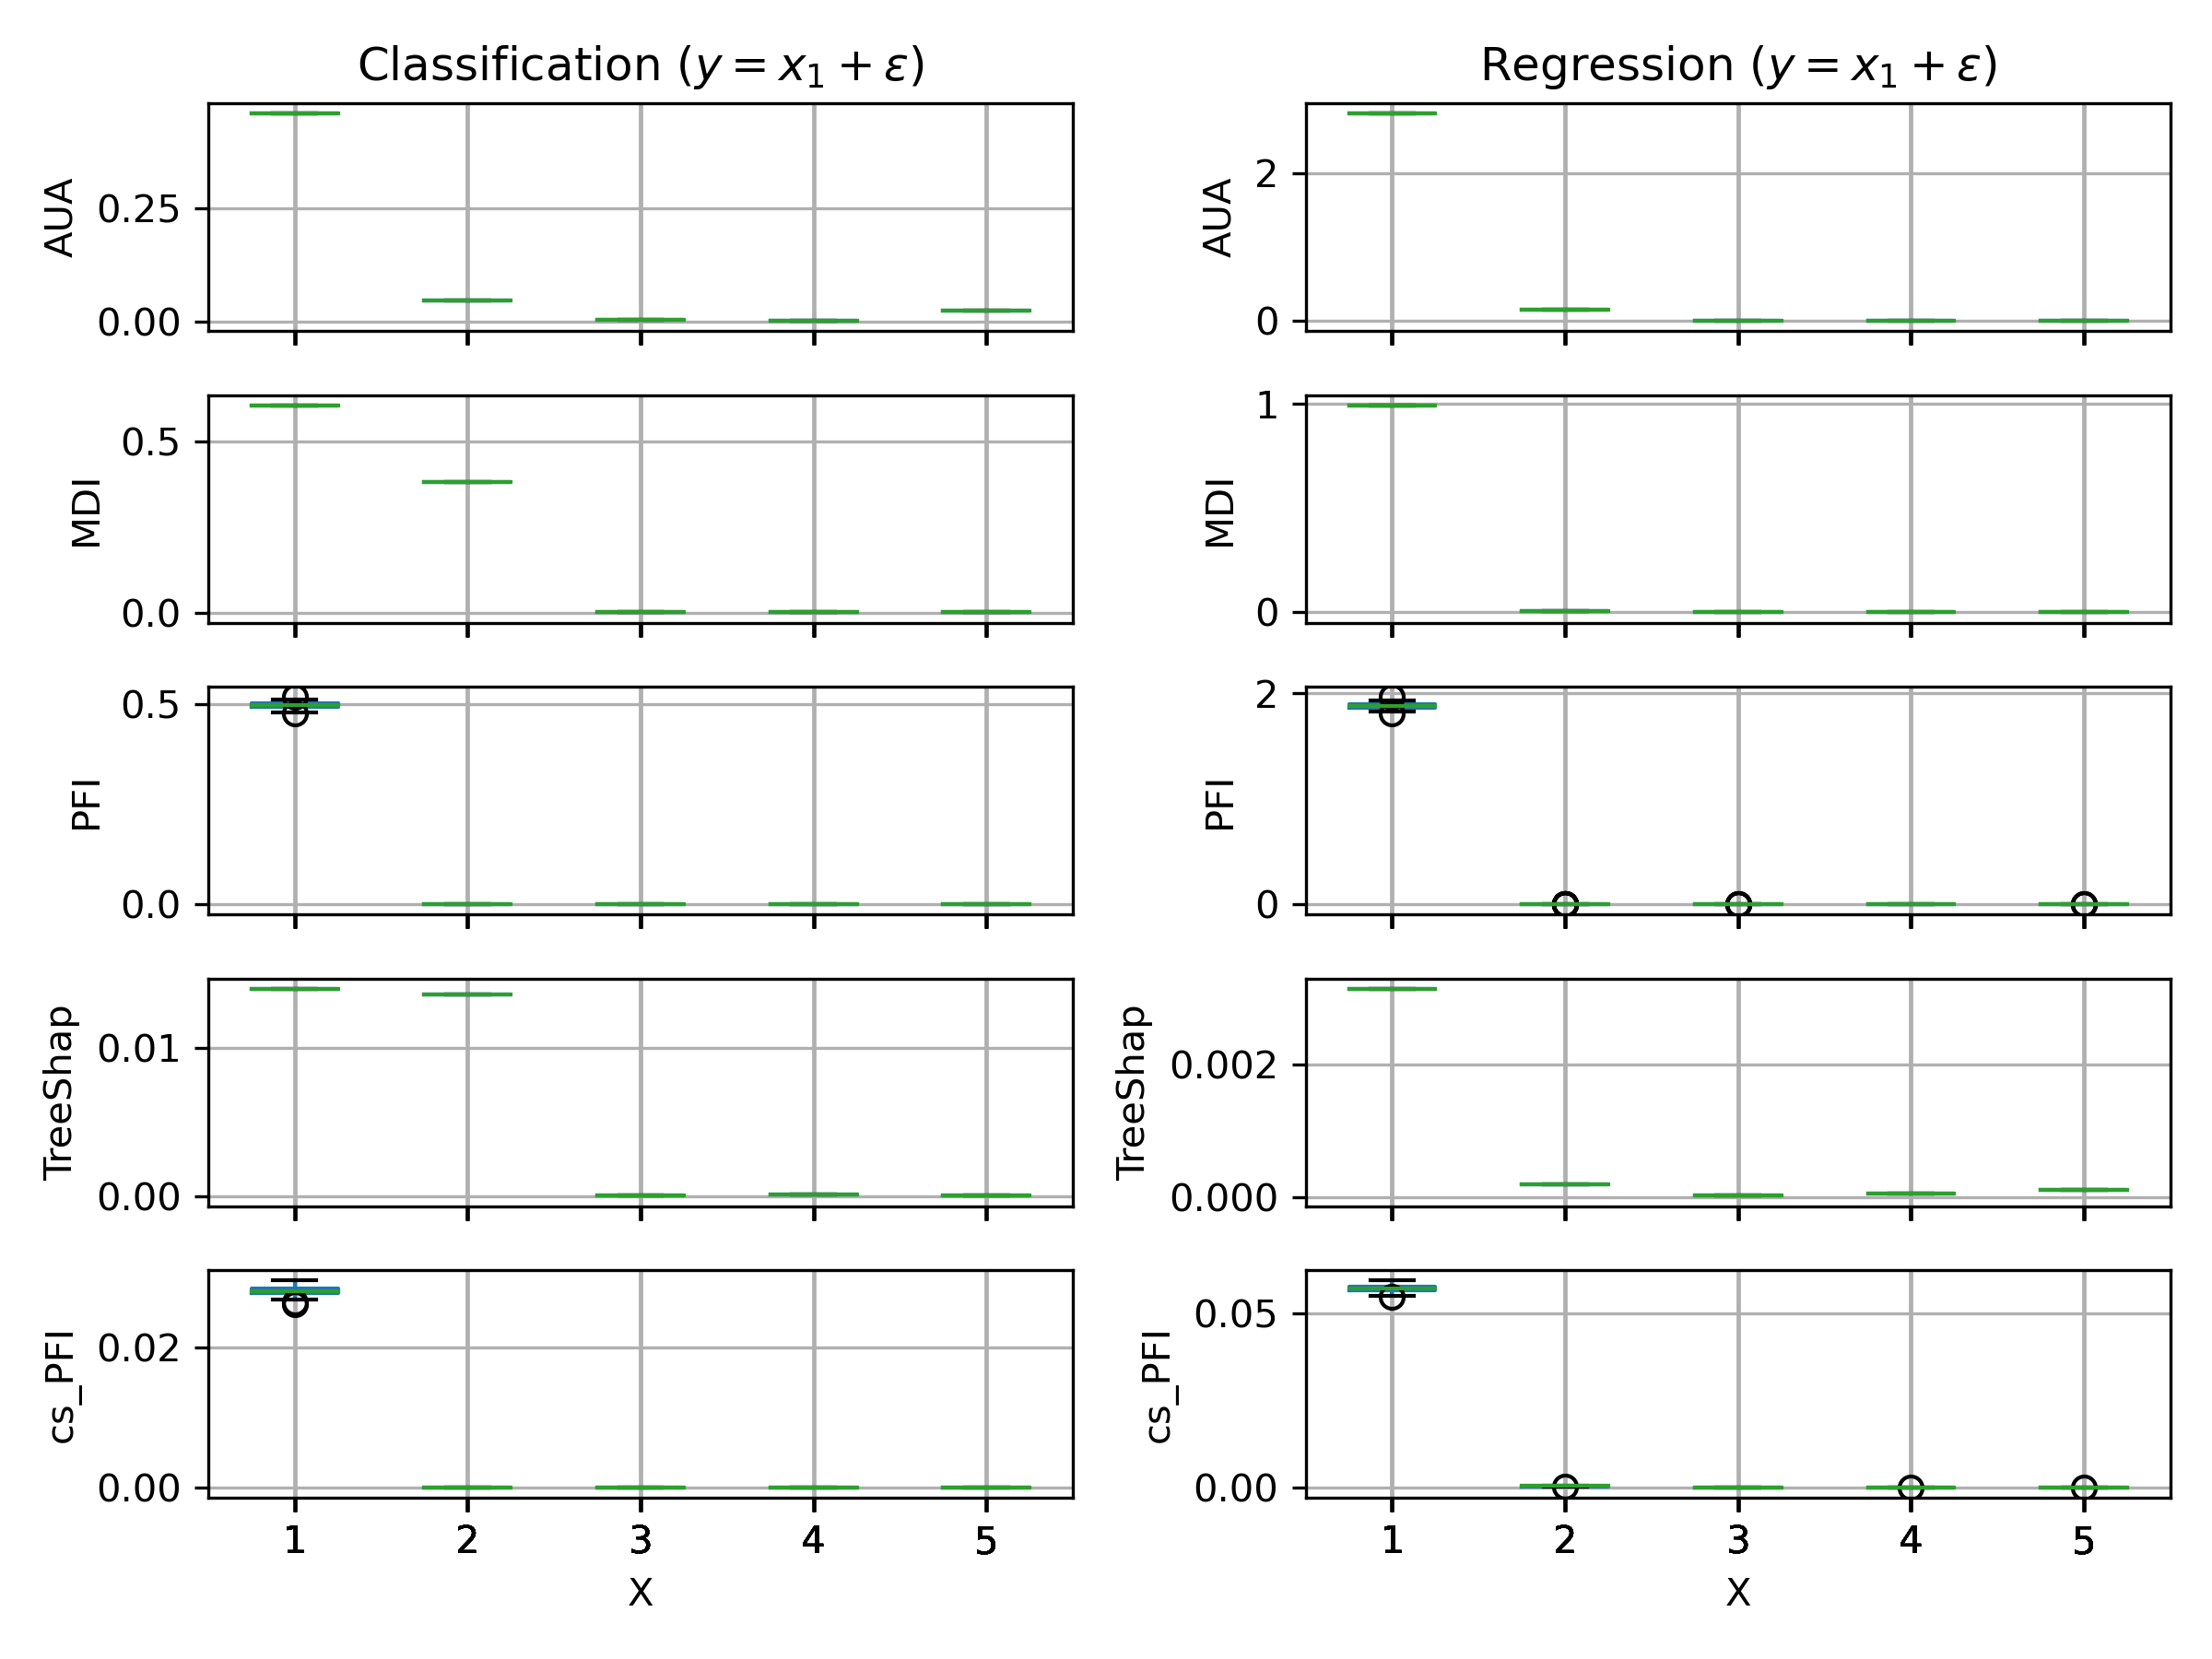
\includegraphics[width=0.98\textwidth]{images/scoreBasedAle/scenario_1_FI.png}}
  \caption{Scenario 1 - Comparison of the ALE-based metric (AUA) with the baseline for the classification and regression task using the random forest model fitted over 100 Monte Carlo replicates.}
    \label{fig:chap5_1}
\end{figure}

With similar results, Figure \ref{fig:scenario2} shows to the \textbf{Scenario 2} how TreeShap and \gls{MDI} give too much relevance for the other correlated feature in the classification task, even though \(y\) depends only on \(x_1\). The \gls{MDI} and \gls{csPFI} correctly assign minimal relevance to the uninformative but dependent variable \(x_2\), whereas \gls{AUA} attributes slightly higher, yet still very low relevance to this variable. This is expected, as \gls{AUA} computes differences in predictions while \gls{PFI} and \gls{csPFI} differences in performance. As only one variable determines outcomes, permuting any other feature does not change performance, although it may introduce some prediction noise. Nevertheless, this noise does not critically affect the recognition of \(x_1\) as the unique key variable to the second scenario. This pattern is evident in the regression task, where all techniques yield satisfactory results. However, techniques that measure changes in predictions, such as TreeShap and \gls{AUA}, do account for some noise in the irrelevant variables. The TreeShap and \gls{MDI} also erroneously attribute so much relevance to the independent and irrelevant variable \(x_5\) in the classification task. 

\begin{figure}[ht!]
\centering
  \fcolorbox{gray}{white}{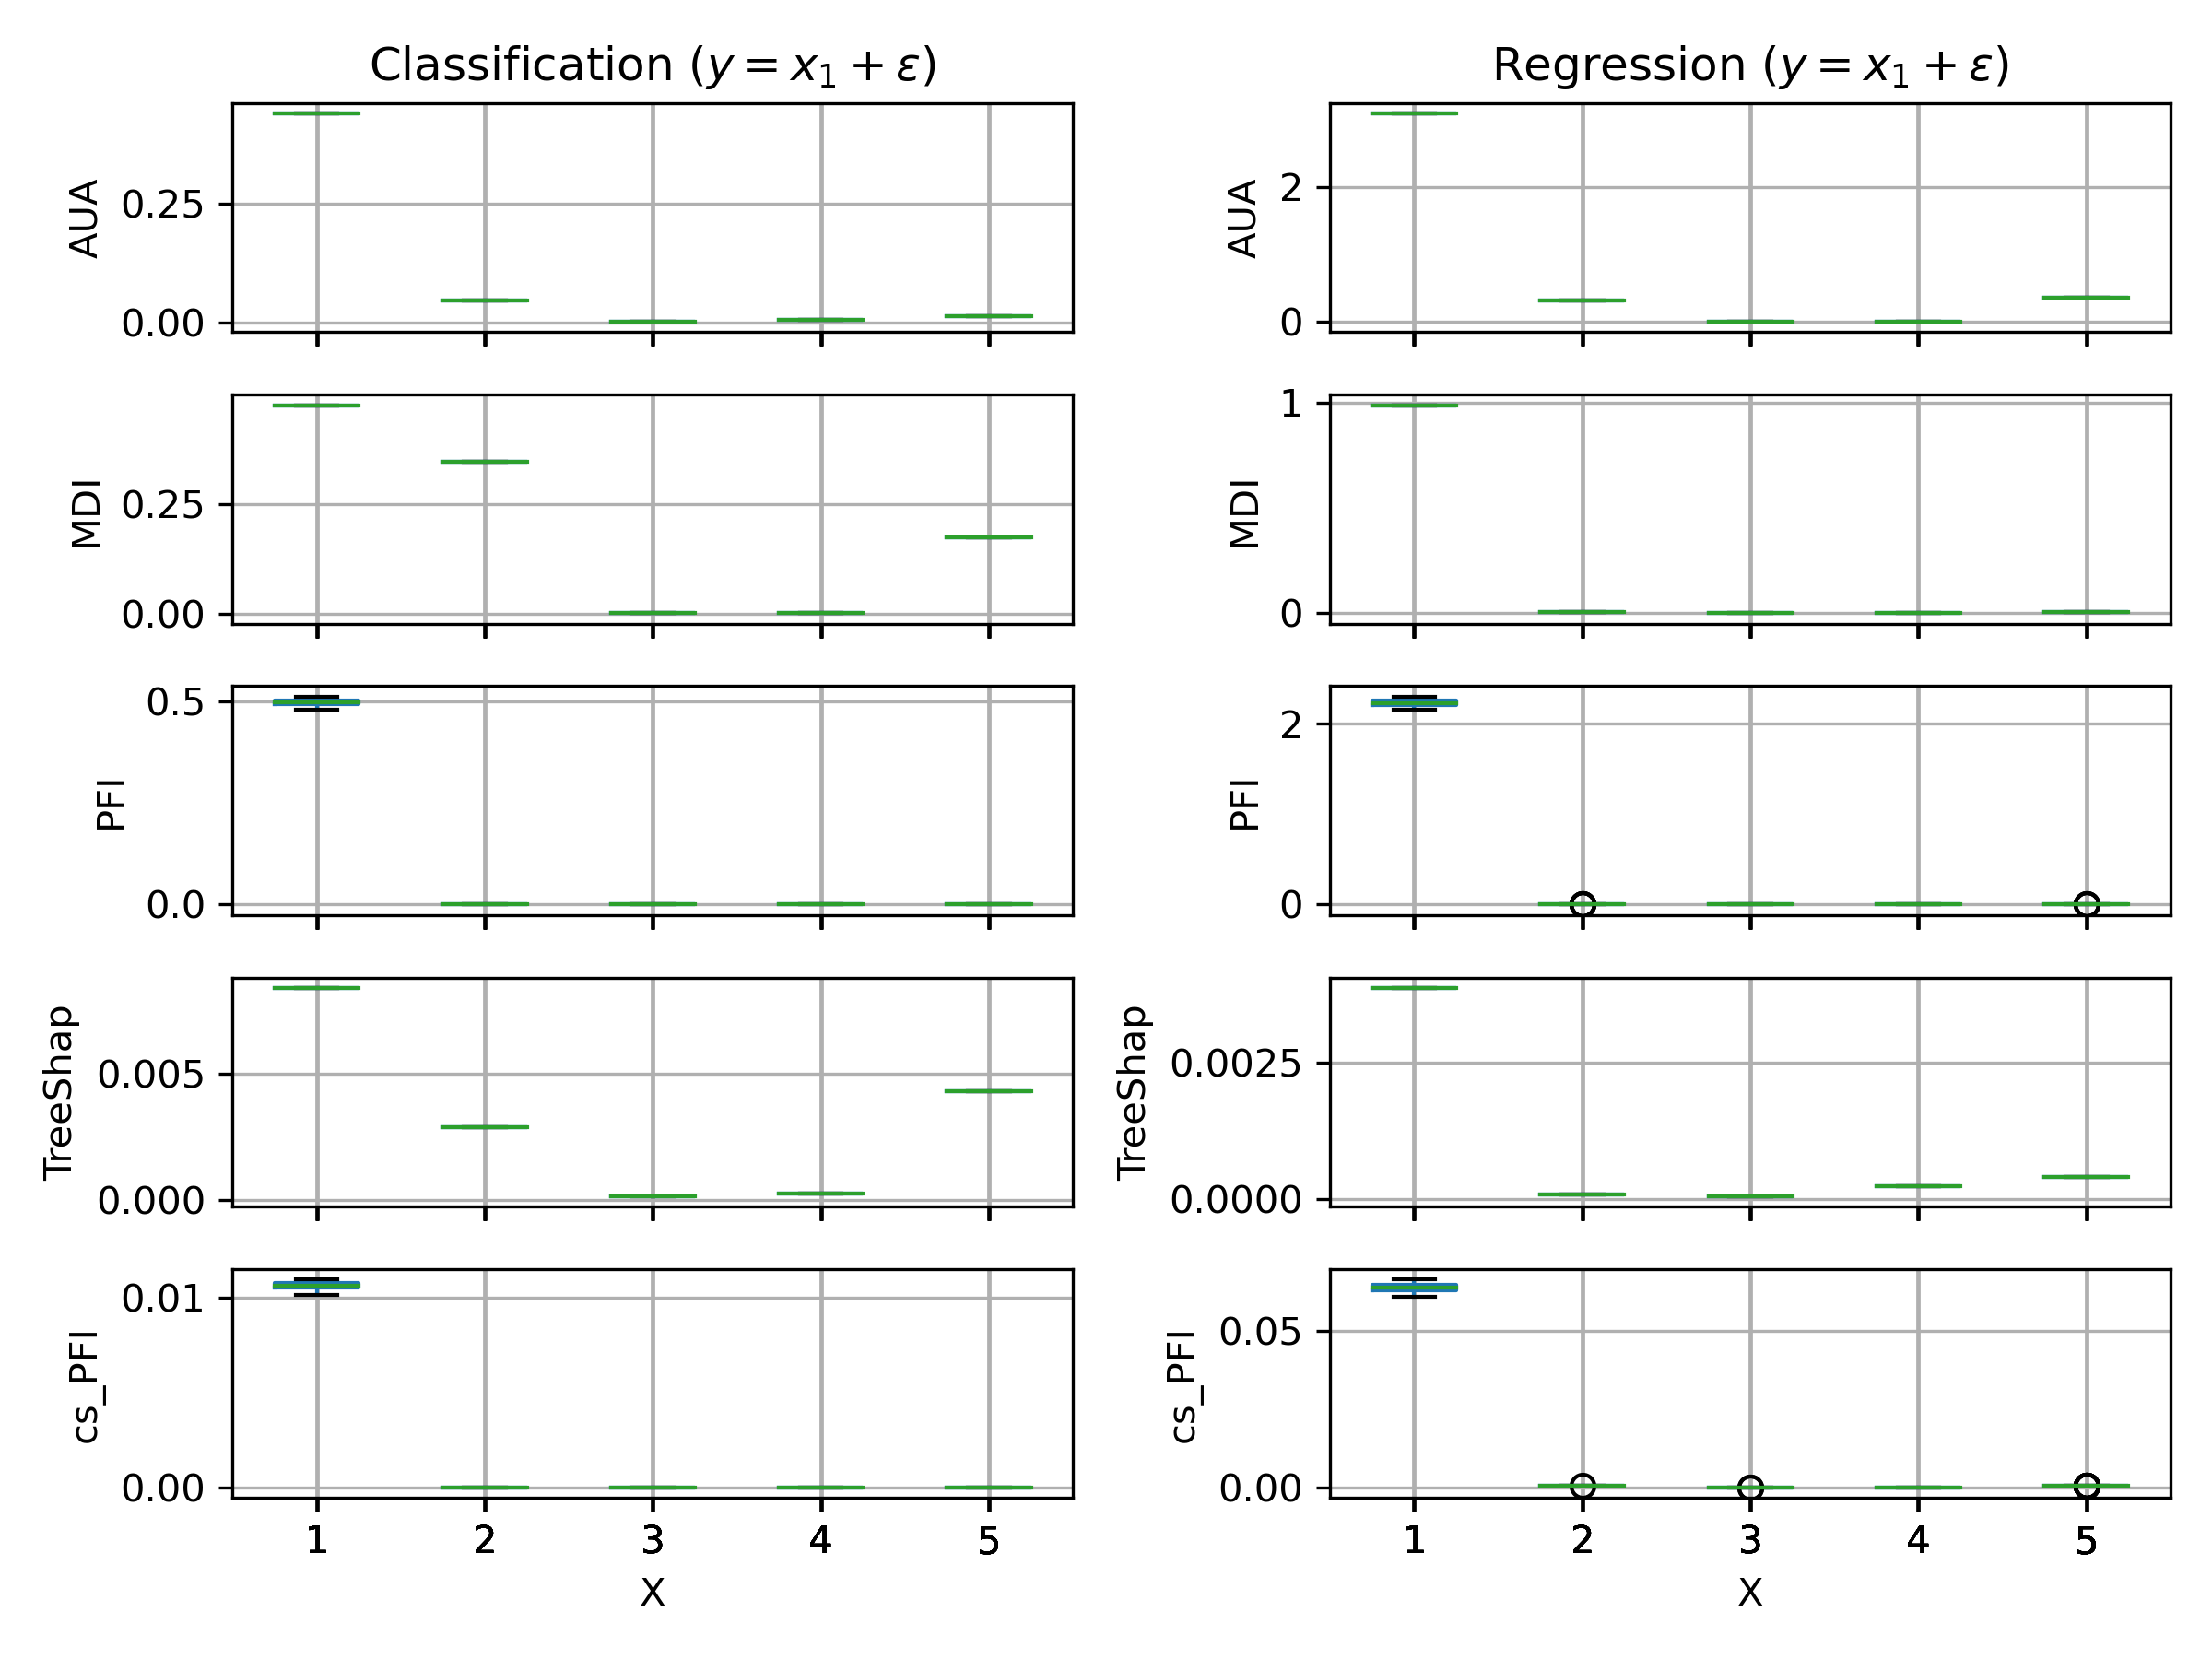
\includegraphics[width=0.98\textwidth]{images/scoreBasedAle/scenario_2_FI.png}}
  \caption{Scenario 2- Comparison of the ALE-based metric (AUA) with the baseline for the classification and regression task using the random forest model fitted over 100 Monte Carlo replicates.}
    \label{fig:scenario2}
\end{figure}

Figure \ref{fig:scenario3} displays the results for \textbf{Scenario 3}. Unlike the second scenario, where a single variable determines the outcome, the target variable \(y\) in the third scenario is influenced by both \(x_1\) and \(x_2\). Given that \(x_1\) is dependent on \(x_2\), \gls{PFI} and \gls{csPFI} encounter difficulties in accurately assessing the relevance of these variables, erroneously favoring one over the other in both classification and regression tasks to \gls{PFI} and only in the regression task for \gls{csPFI}. Conversely, TreeSHAP, \gls{MDI}, and \gls{AUA} yield more accurate feature relevance rankings. However, in the classification task, both \gls{AUA} and \gls{MDI} incorrectly attribute some importance to the feature \(x_5\), which, although highly correlated with \(x_1\), has no direct influence on \(y\). The error is more critical for \gls{MDI}, which assigns approximately half the relevance to \(x_5\) as it does to \(x_1\), whereas \gls{AUA} erroneously assigns a notably lower relevance.


\begin{figure}[ht!]
\centering
  \fcolorbox{gray}{white}{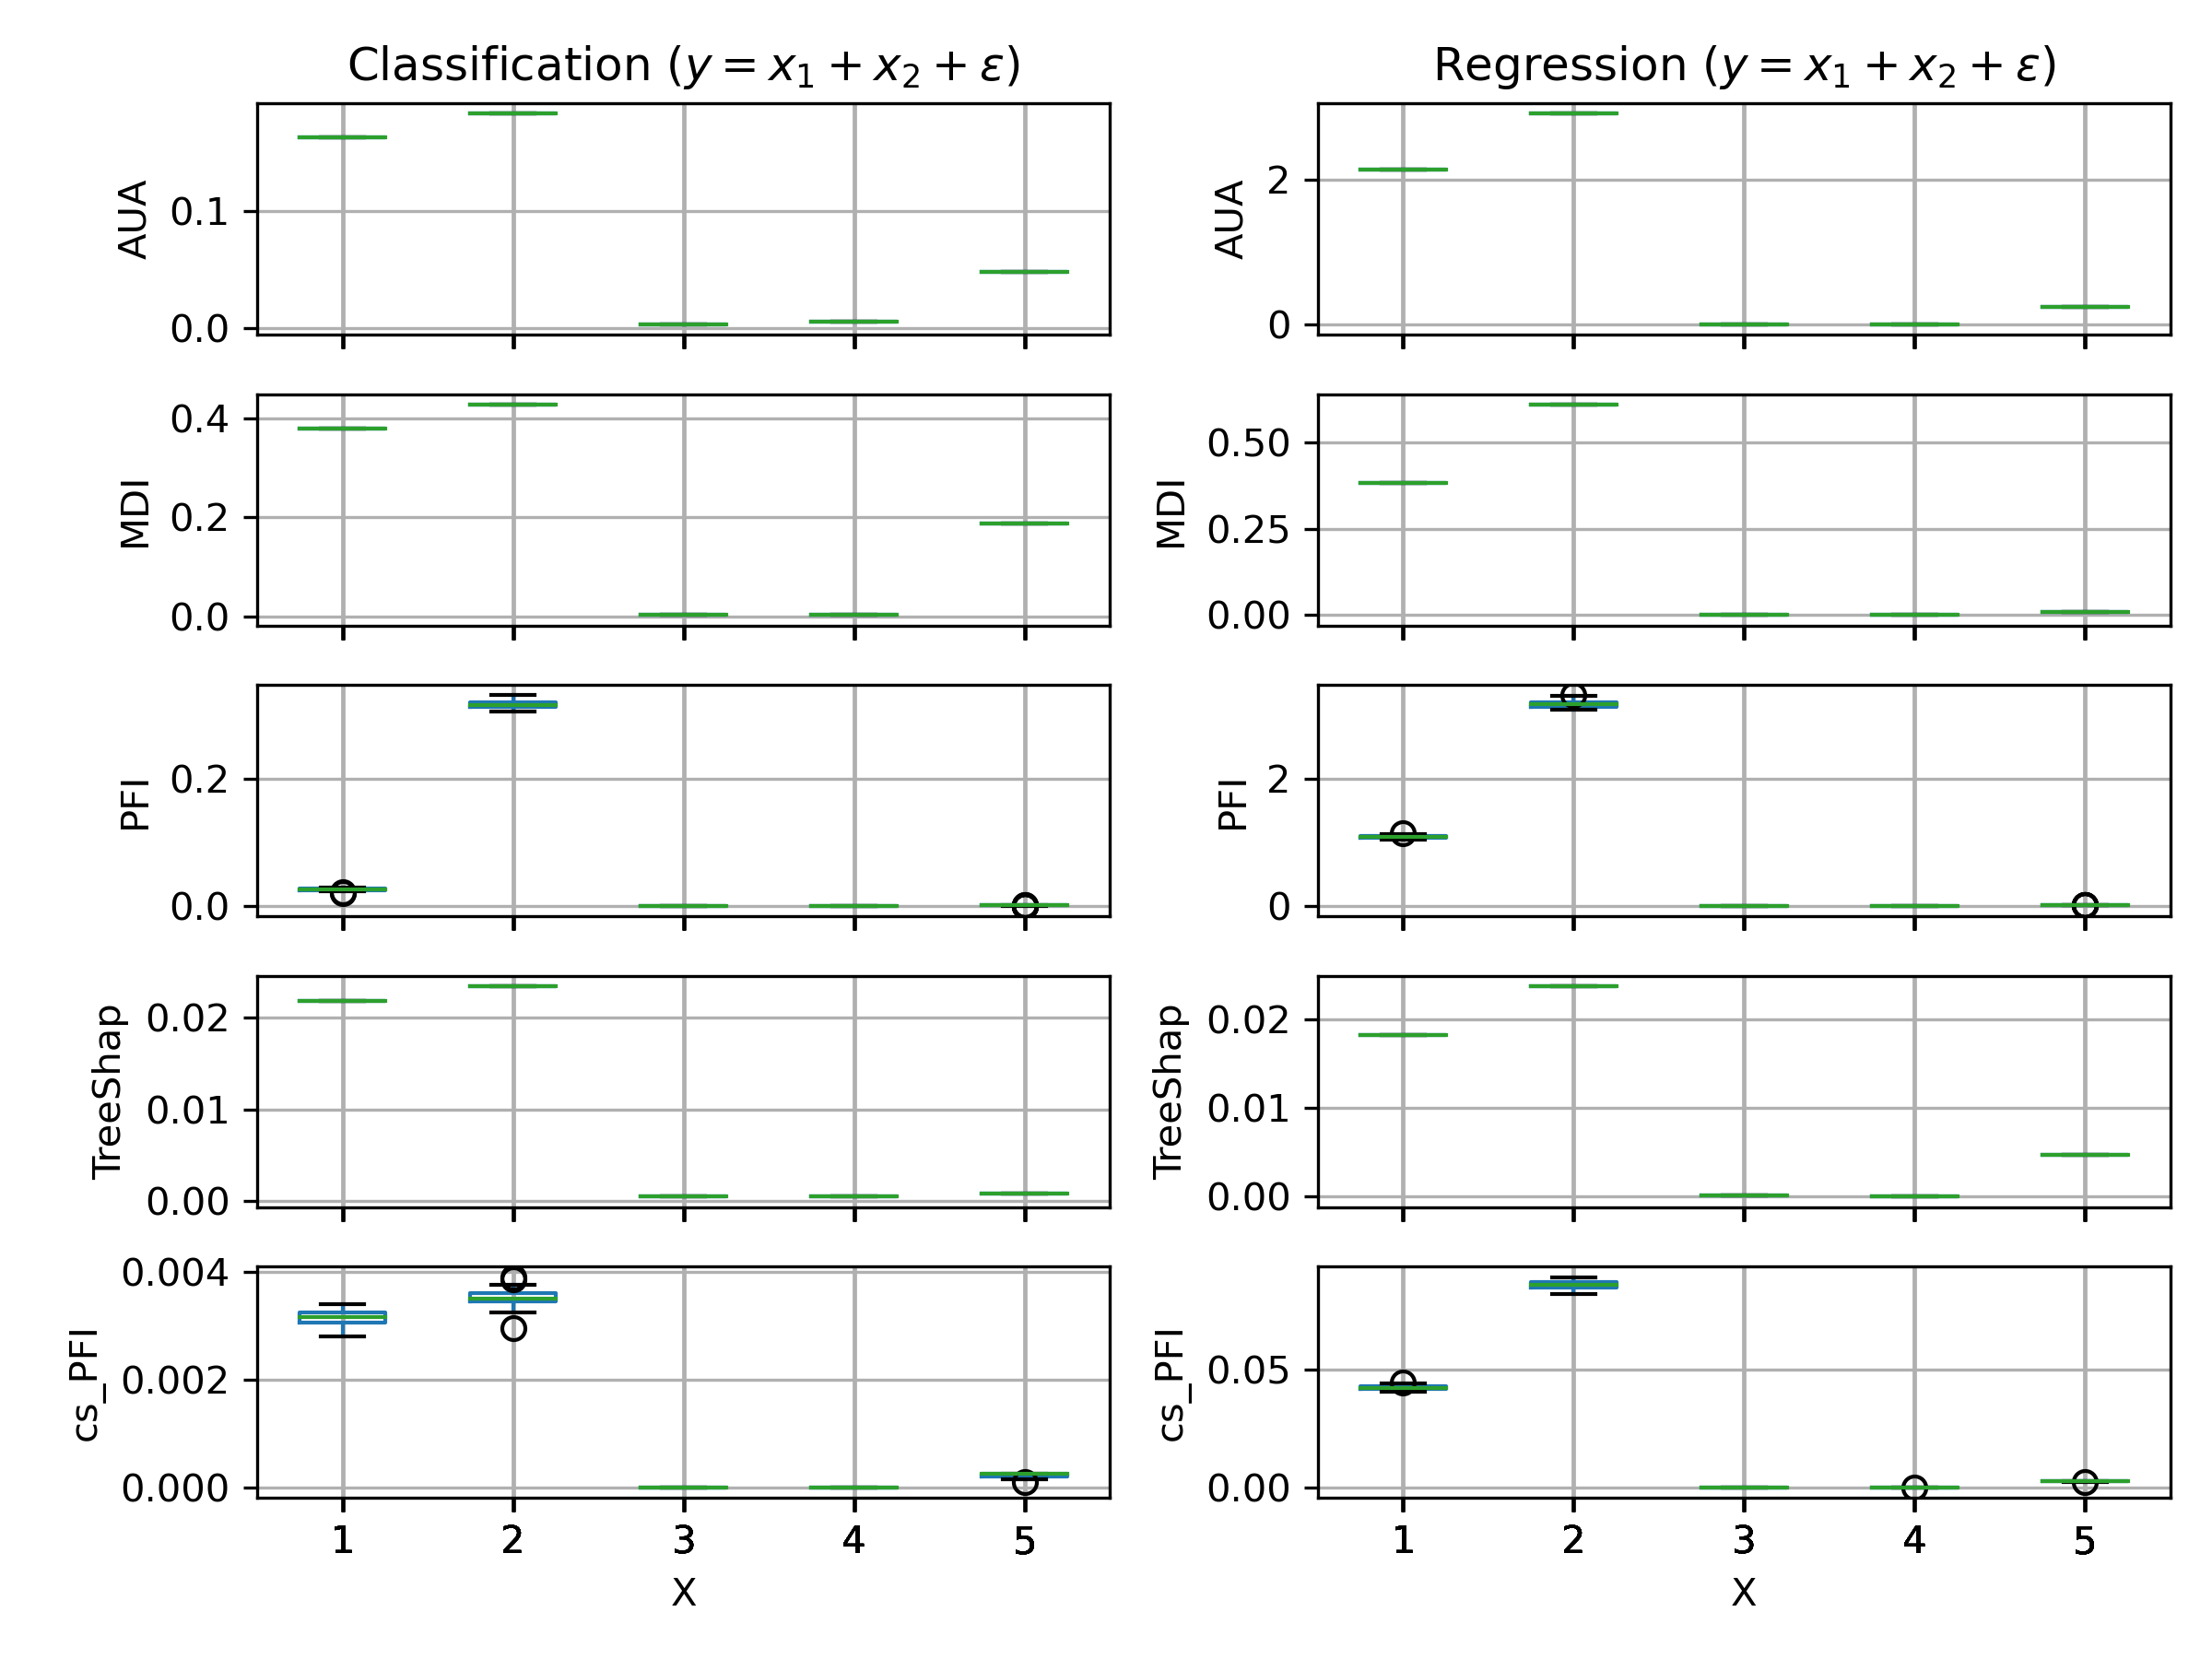
\includegraphics[width=0.98\textwidth]{images/scoreBasedAle/scenario_3_FI.png}}
  \caption{Scenario 3 - Comparison of the ALE-based metric (AUA) with the baseline for the classification and regression task using the random forest model fitted over 100 Monte Carlo replicates.}
    \label{fig:scenario3}
\end{figure}

\subsubsection{Quantitative analysis}

Figure \ref{fig:propTrueVar} shows how the performance of methods changes to the \textit{PropTrueVar} as the Pearson correlation between variables escalates from 0.1 to 0.8 as defined in \textbf{Scenario 4}.

A \textit{PropTrueVar} value approaching 1 signifies an effective technique in assigning higher relevance to the true explanatory variable, whereas a value substantially deviating from 1 indicates a less reliable method. Figure \ref{fig:propTrueVar} corroborates previous findings, revealing a more robustness of \gls{PFI}, \gls{csPFI} and the ALE-based (\gls{AAR}) across interactions, while \gls{MDI} and TreeSHAP fail to identity and isolate the effects of the unique relevant variable \(x_1\) as the level o colinearity increase. Also, TreeSHAP shows a high variability in this simple setting, probably due to its strategy to handle the conditional expectation based on the branch of trees. 

\begin{figure}[ht!]
\centering
  \fcolorbox{gray}{white}{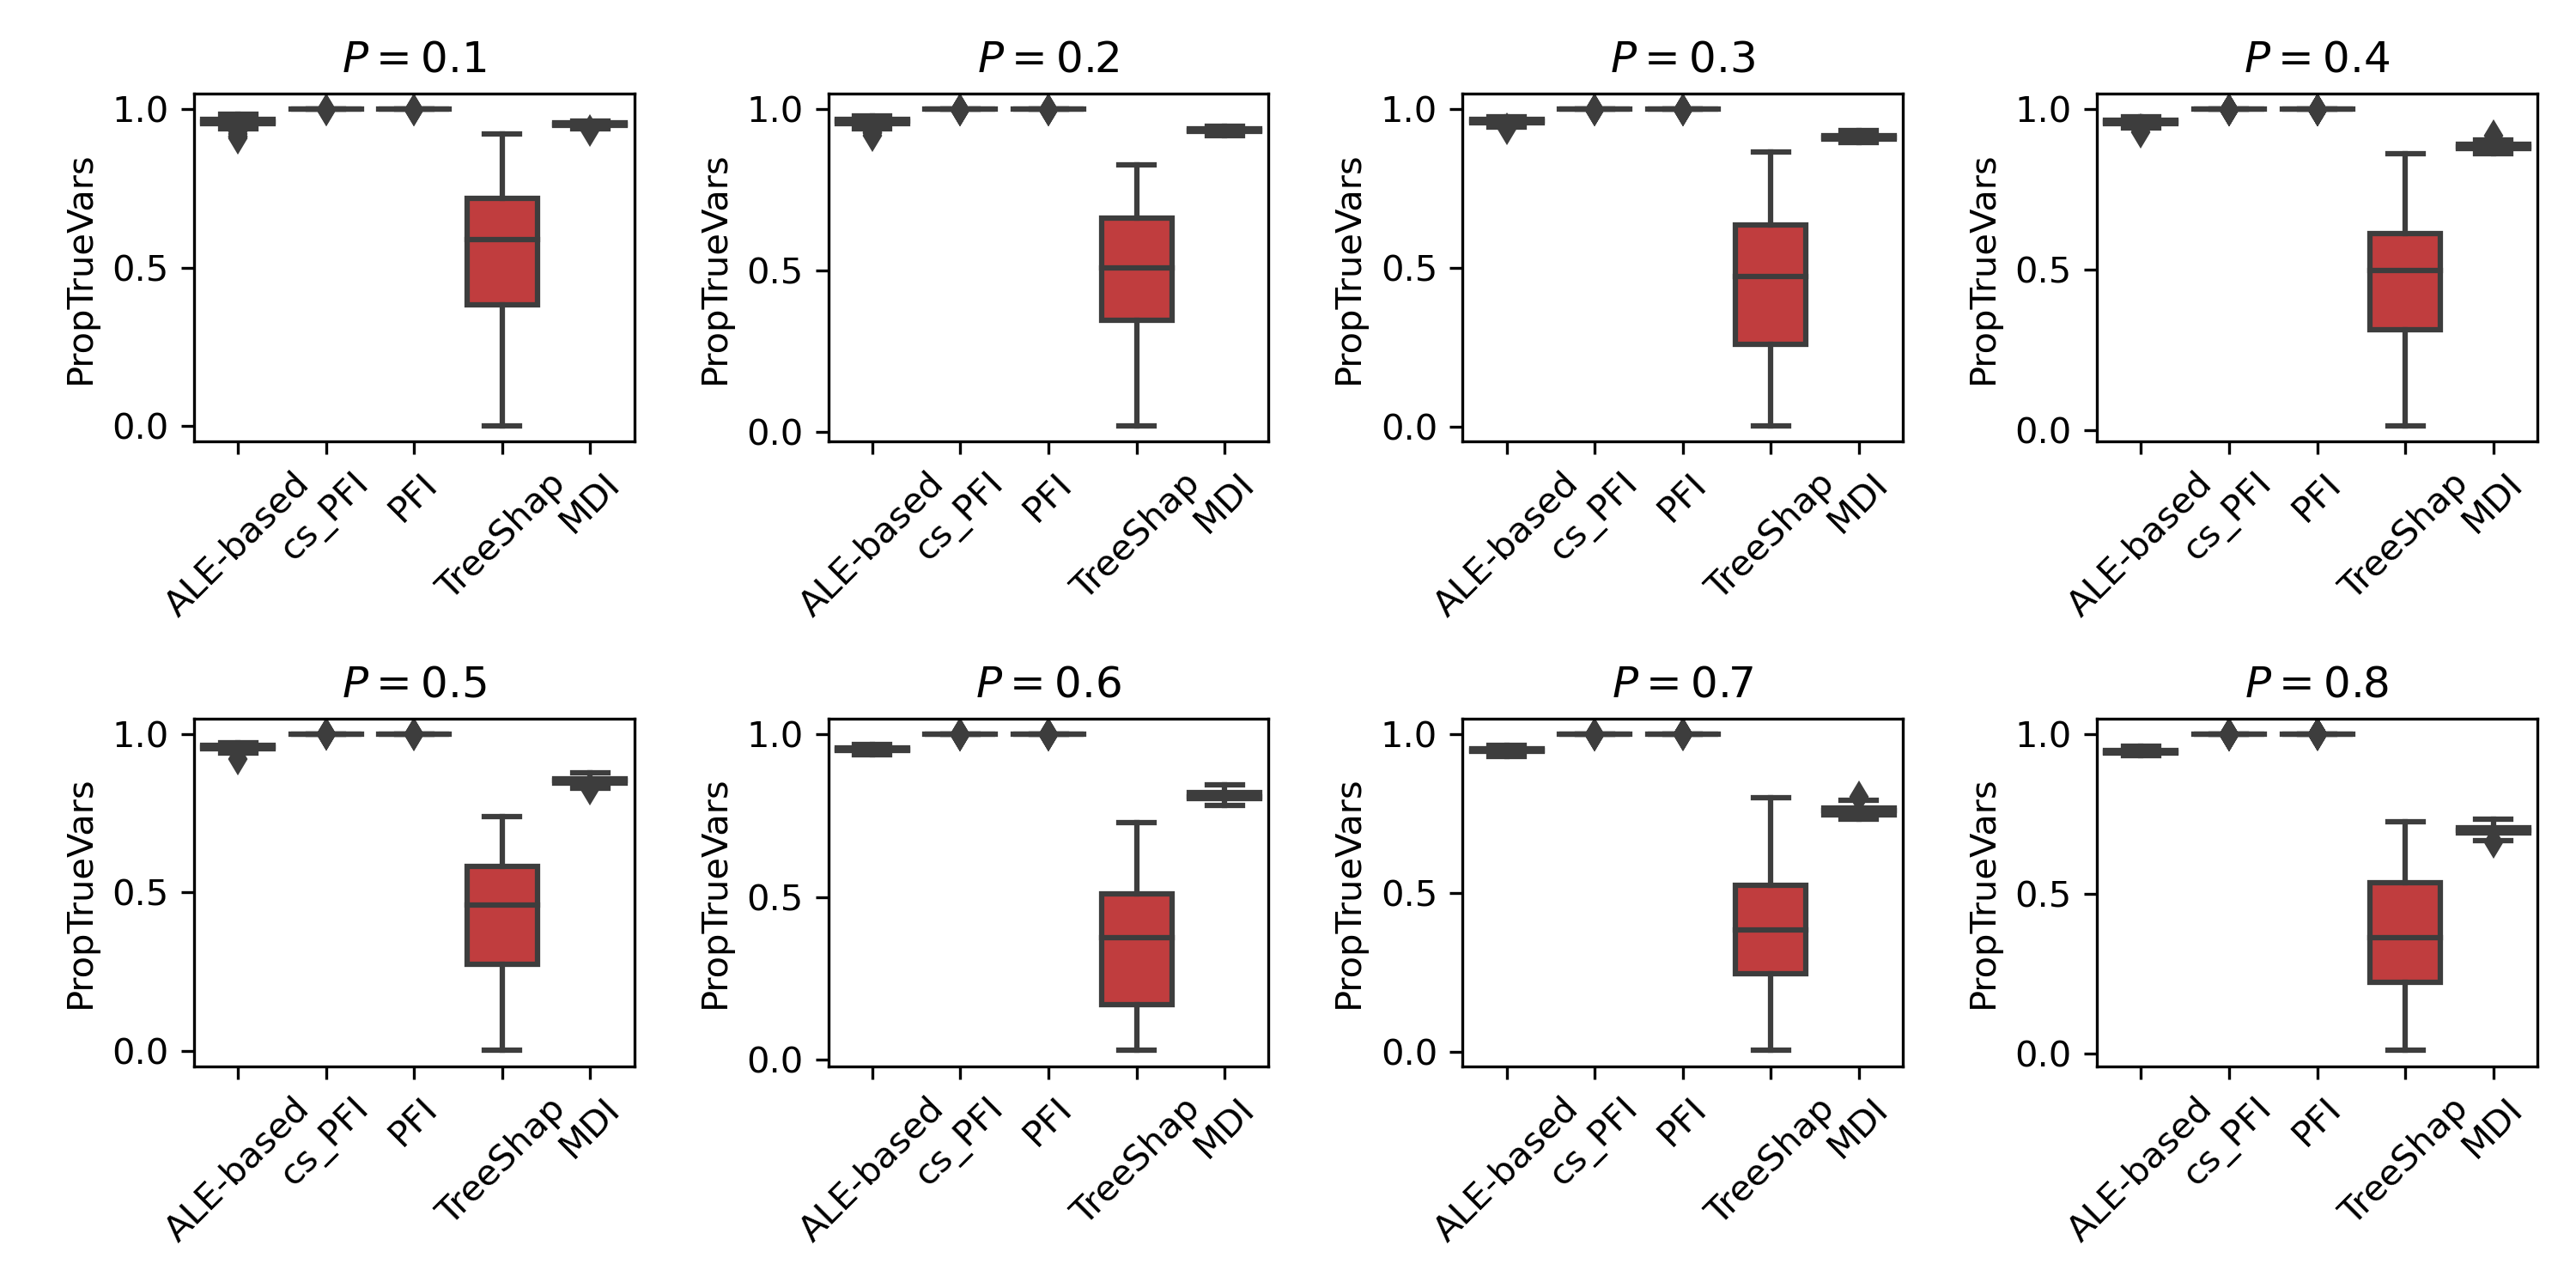
\includegraphics[width=0.98\textwidth]{images/scoreBasedAle/PropTrueVars_box_plot.png}}
  \caption{Scenario 4 - The performance for the metric PropTrueVar across different levels of correlation between the true, relevant variable, and irrelevant variables. PropTrueVar measures the proportion of total relevance attributed to all variables that are assigned for the true relevant variable. The \gls{PFI}, \gls{csPFI}, and ALE-based scores achieve better results when the correlation is high (after 0.6).}
    \label{fig:propTrueVar}
\end{figure}

Figure \ref{fig:equitruevar} illustrates the method's performance on \textit{EquiTrueVar} using \textbf{Scenario 5}. \gls{PFI} achieves the worst results due to its difficulty in highlighting two important variables when they are not independent. The ALE-based score shows great performance at all measured levels of feature dependence. The superiority of the ALE-based method is also evident in \textbf{Scenario 6} when assessing the \textit{EquiPropTrueVars}. The \textit{EquiPropTrueVars} measures a scenario in which the correlation between relevant \(G_1\) and irrelevant variables \(G_2\) increases, alongside the correlation within \(G_1\) variables. Figure \ref{fig:propequitruevar} illustrates the superior performance of the ALE-based approach (\gls{AAR}) across almost all values of intra- and inter-correlations. The performance with respect to \textit{EquiPropTrueVars} diminishes when the intra-dependence within \(G_1\) becomes critically high, while the dependence between \(G_1\) and \(G_2\) appears to have a lesser impact on the proposed metric. However, in nearly all configurations, the ALE method achieves the best results.

\begin{figure}[ht!]
\centering
  \fcolorbox{gray}{white}{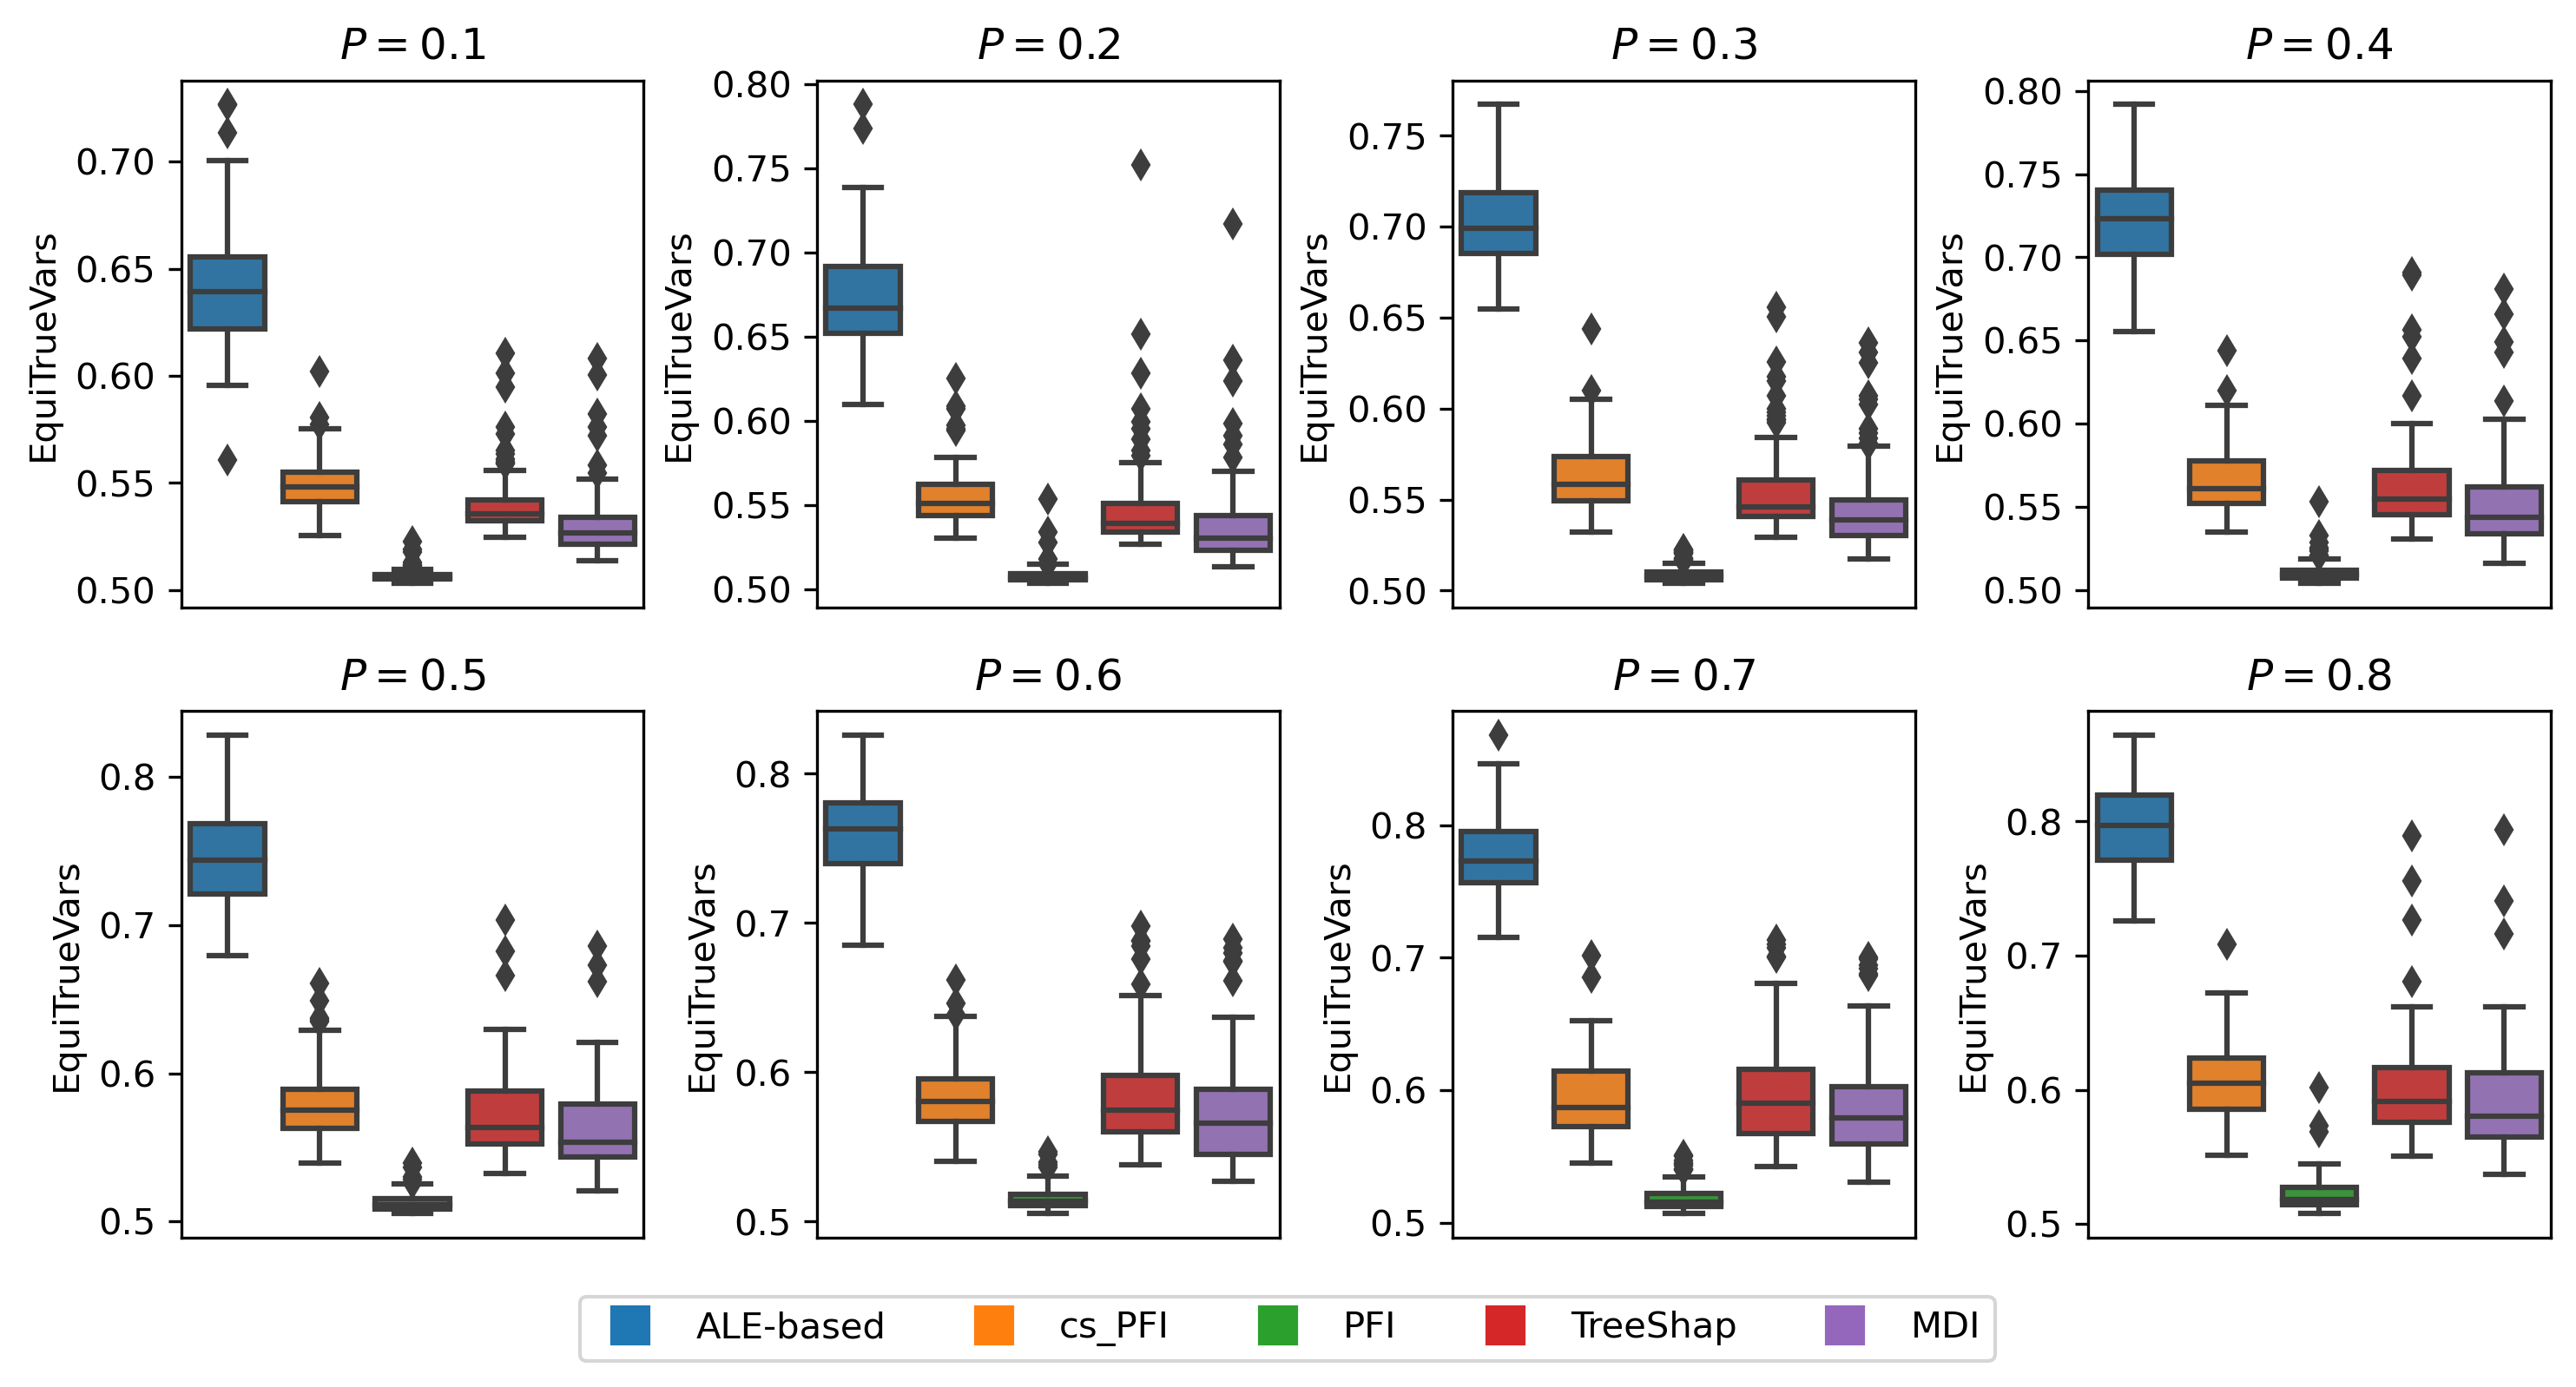
\includegraphics[width=0.98\textwidth]{images/scoreBasedAle/EquiTrueVars.png}}
  \caption{Scenario 5- The performance for the metric \textit{EquiTrueVar} across different levels of correlation between the two true relevant variables. The ALE-based scores achieve better results.}
    \label{fig:equitruevar}
\end{figure}


\begin{figure}[ht!]
\centering
  \fcolorbox{gray}{white}{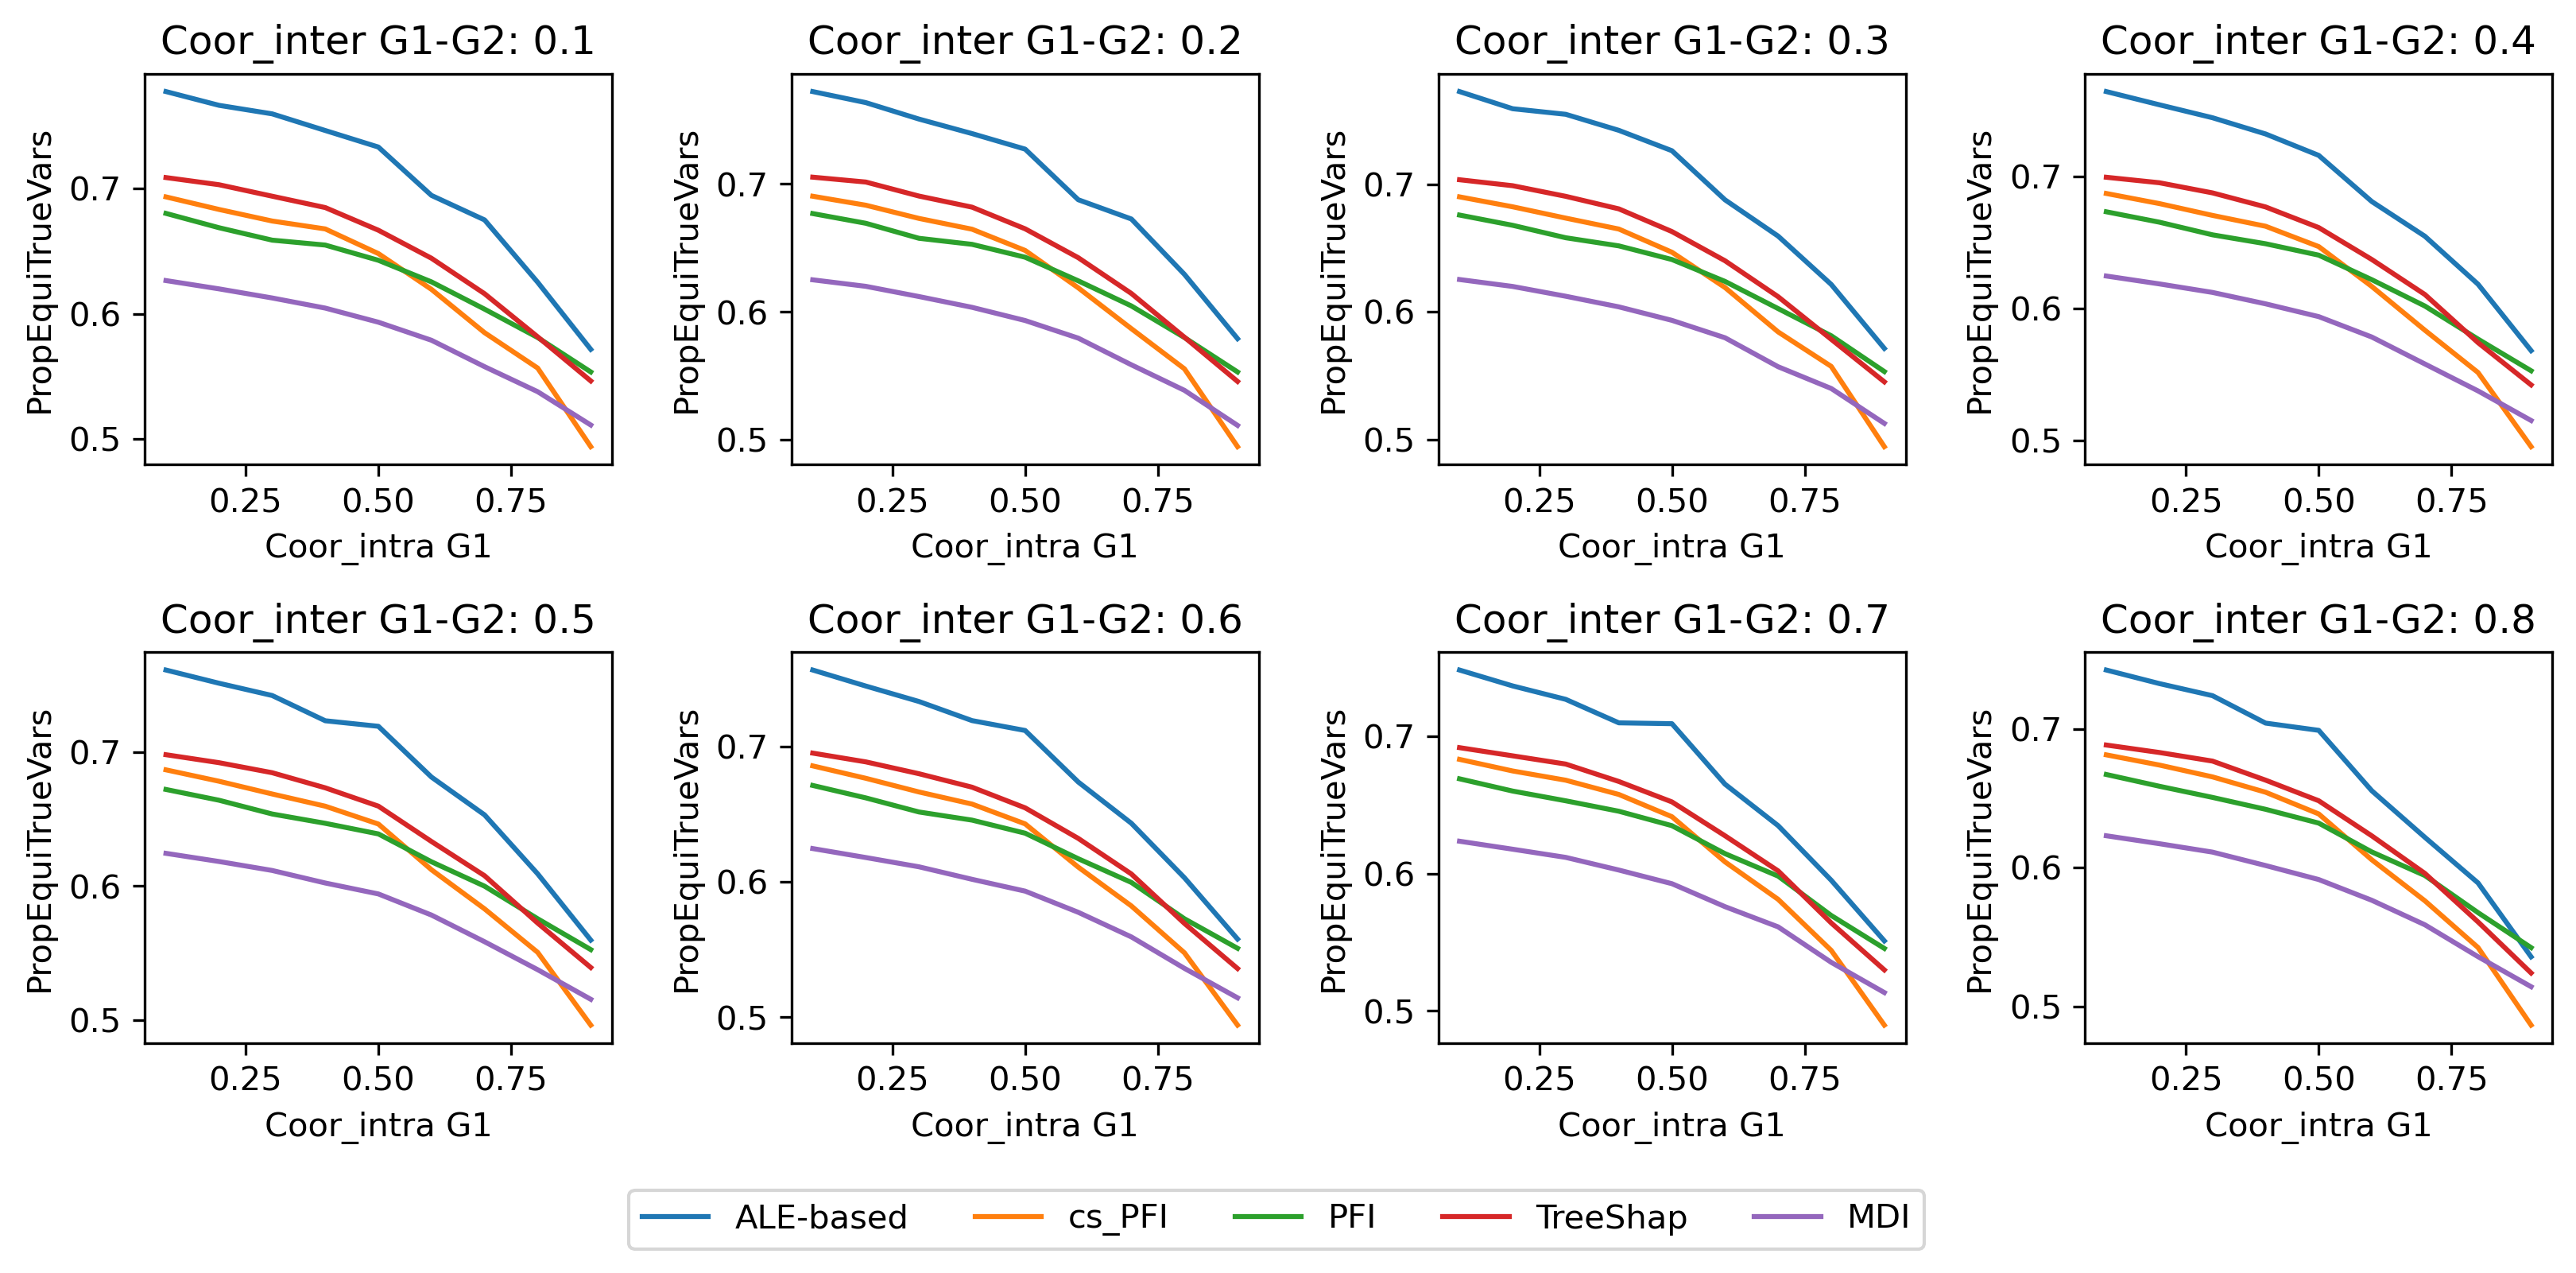
\includegraphics[width=0.98\textwidth]{images/scoreBasedAle/PropEquiTrueVars.png}}
  \caption{Scenario 6- The performance for the metric \textit{EquiPropTrueVar} across different levels of correlation between relevant variables and irrelevant variables as well as within the relevant variables. The ALE-based scores achieve better results for almost all settings.}
    \label{fig:propequitruevar}
\end{figure}

\subsection{Real-world data}

The results for the cancer dataset are depicted in Figure \ref{fig:cancer}. The red bars represent the top 10 features as determined by each metric. Intriguingly, the strong interdependence among many variables in this dataset highlights the limitations of permutation-based metrics such as \gls{csPFI} and \gls{PFI}, which depend on differences in model error for their calculations. Looking at the absolute value of feature effects size, these metrics suggest that almost none of the features are relevant, as evidenced by the assignment of values close to zero. There are numerous variables with zero effect, and no variable changes the model accuracy by more than \(2 x 10^-3\) in \gls{csPFI} and \(2 x 10^-2\) in \gls{PFI}. 

While \gls{csPFI} and \gls{PFI} metrics have good results for PropTrueVar - where only one variable was relevant -  in the previous experiment, they are unable to distinguish the impact of individual variables in the current scenario due to the high degree of interdependence among variables, as is evident in Figure \ref{fig:correlation}. To make it clear, all metrics were arranged in a ranking-based setting. In the case of the ALE-based score, the AAR was utilized, and for TreeSHAP, the absolute average method was employed. Unlike \gls{PFI} and \gls{csPFI}, the \gls{AAR}, \gls{MDI}, and TreeSHAP, despite some discrepancies, consistently identify many relevant features with a similar set of features within the top 10.

\begin{figure}[ht!]
\centering
  \fcolorbox{gray}{white}{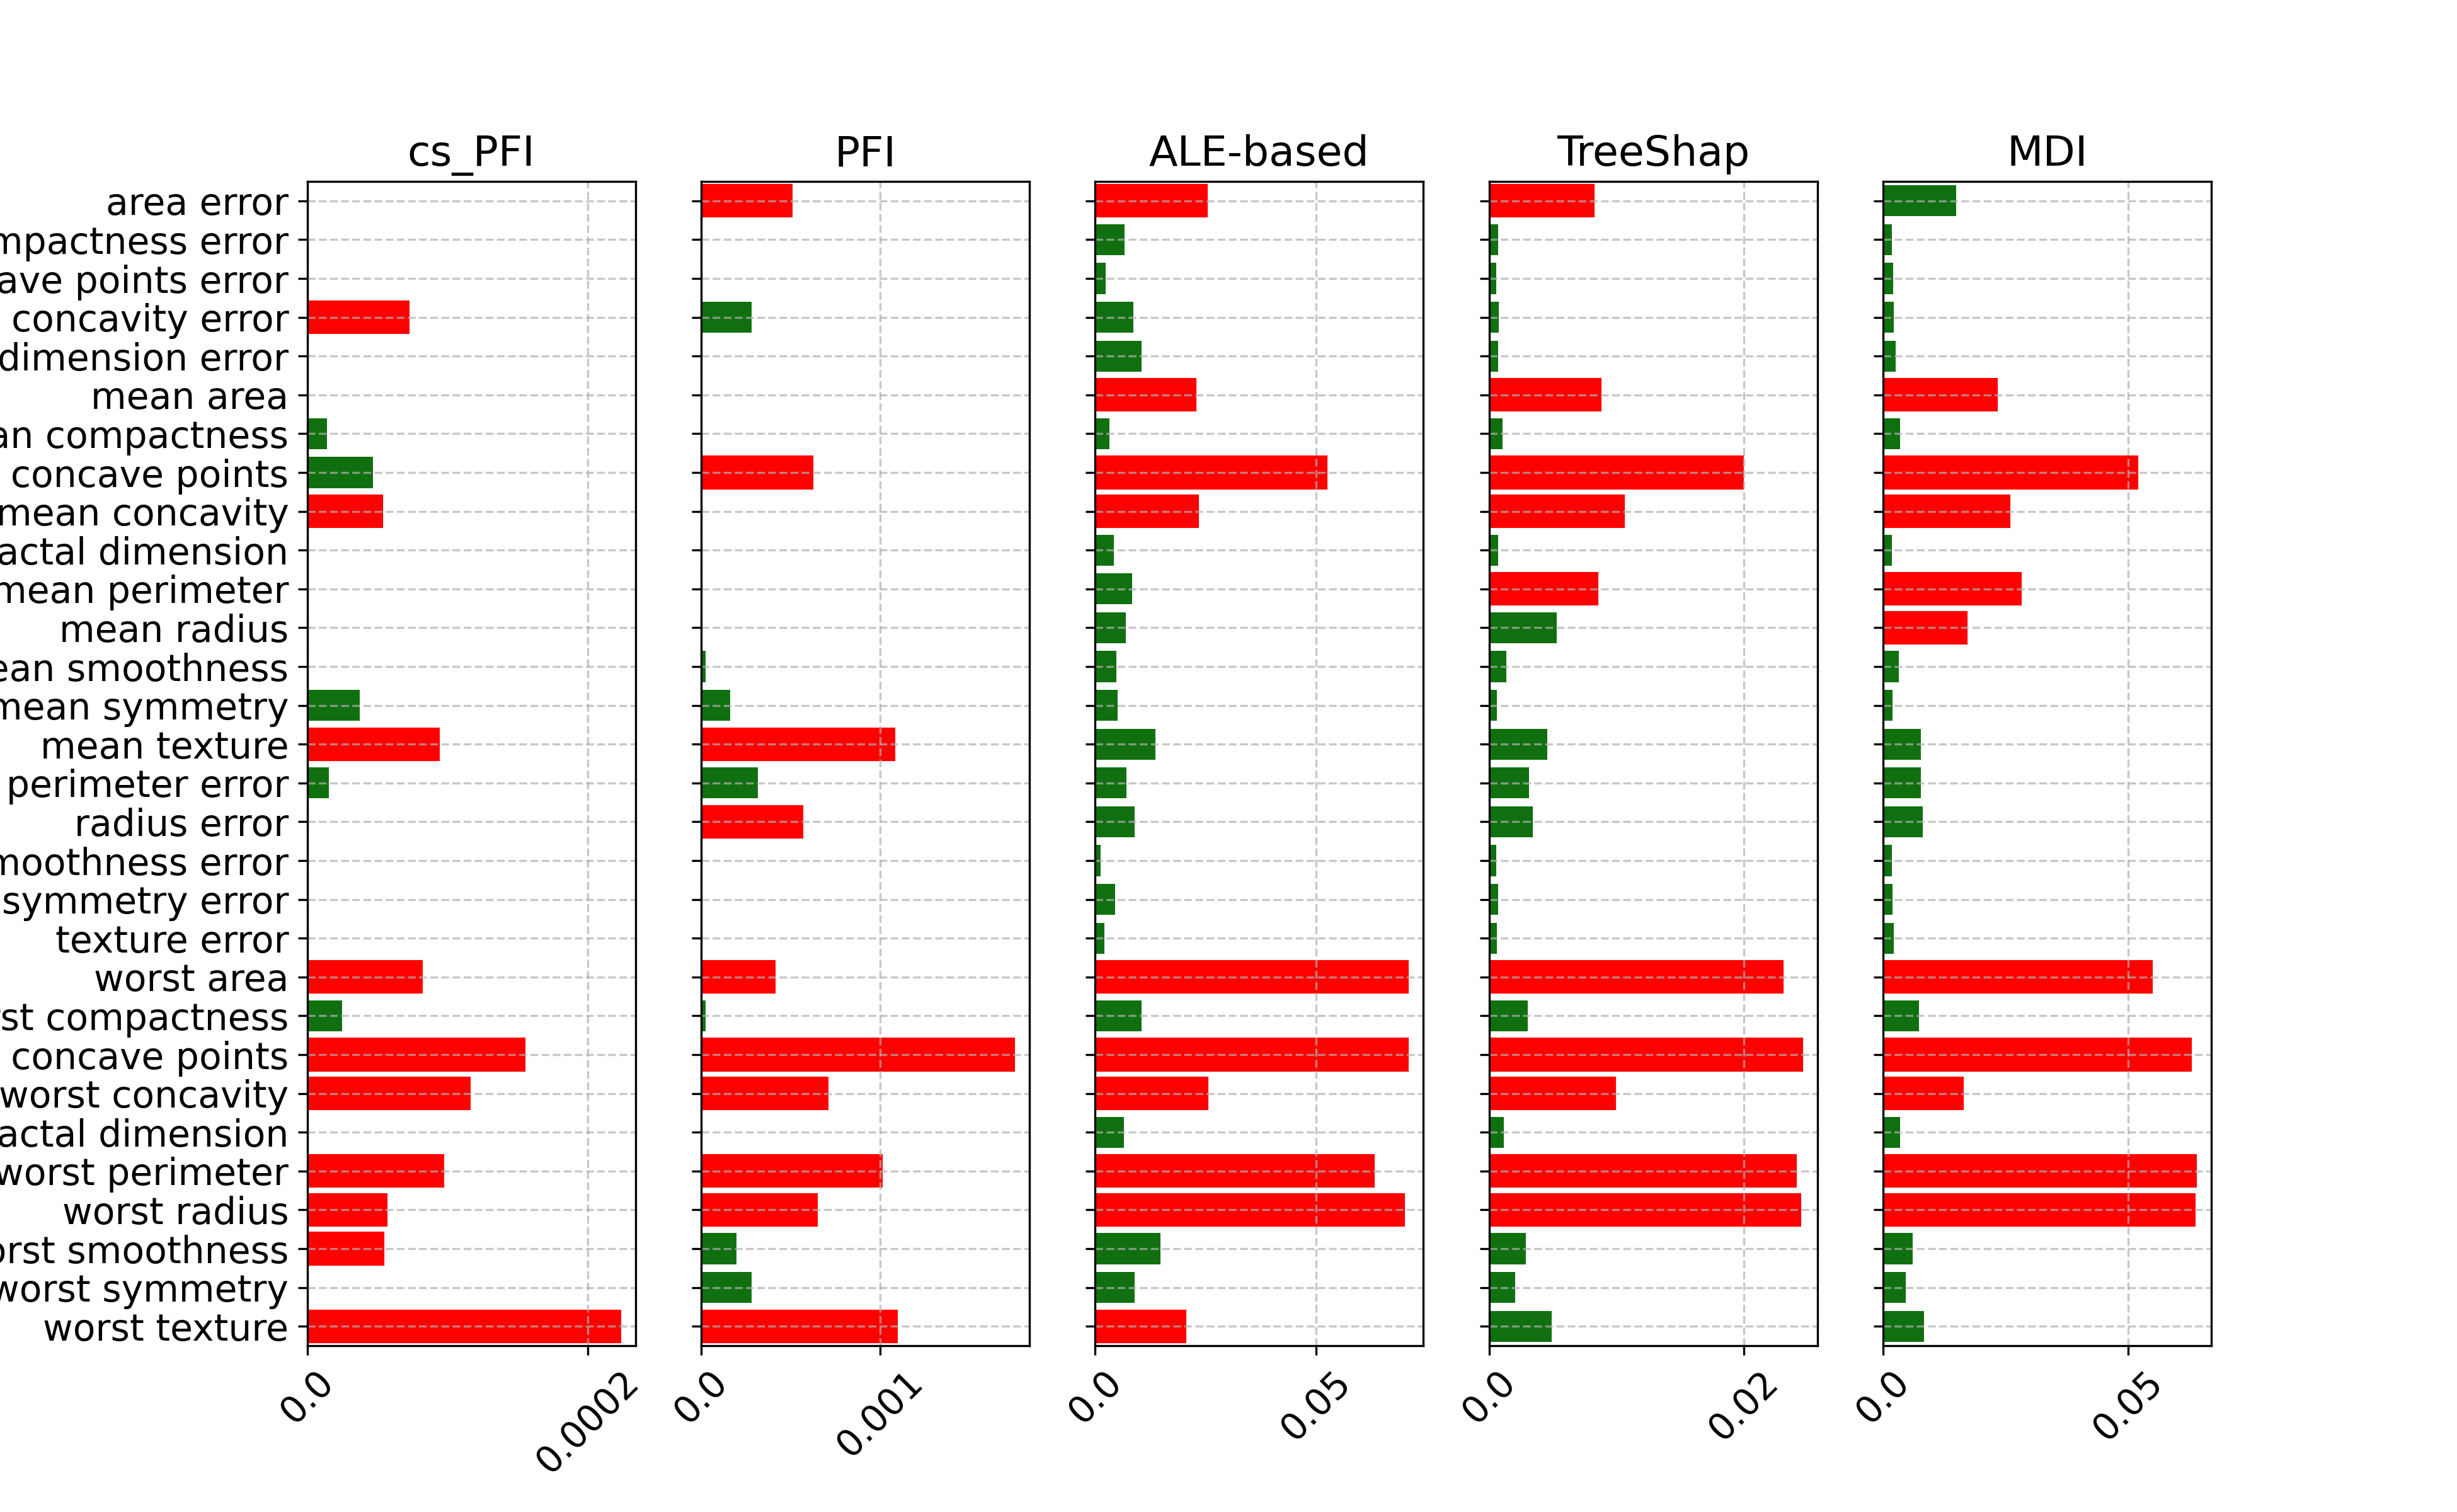
\includegraphics[width=0.98\textwidth]{images/scoreBasedAle/cancer_data.png}}
  \caption{Cancer data - Red bars represent the top 10 features determined by each metric.}
    \label{fig:cancer}
\end{figure}

\begin{figure}[ht!]
\centering
  \fcolorbox{gray}{white}{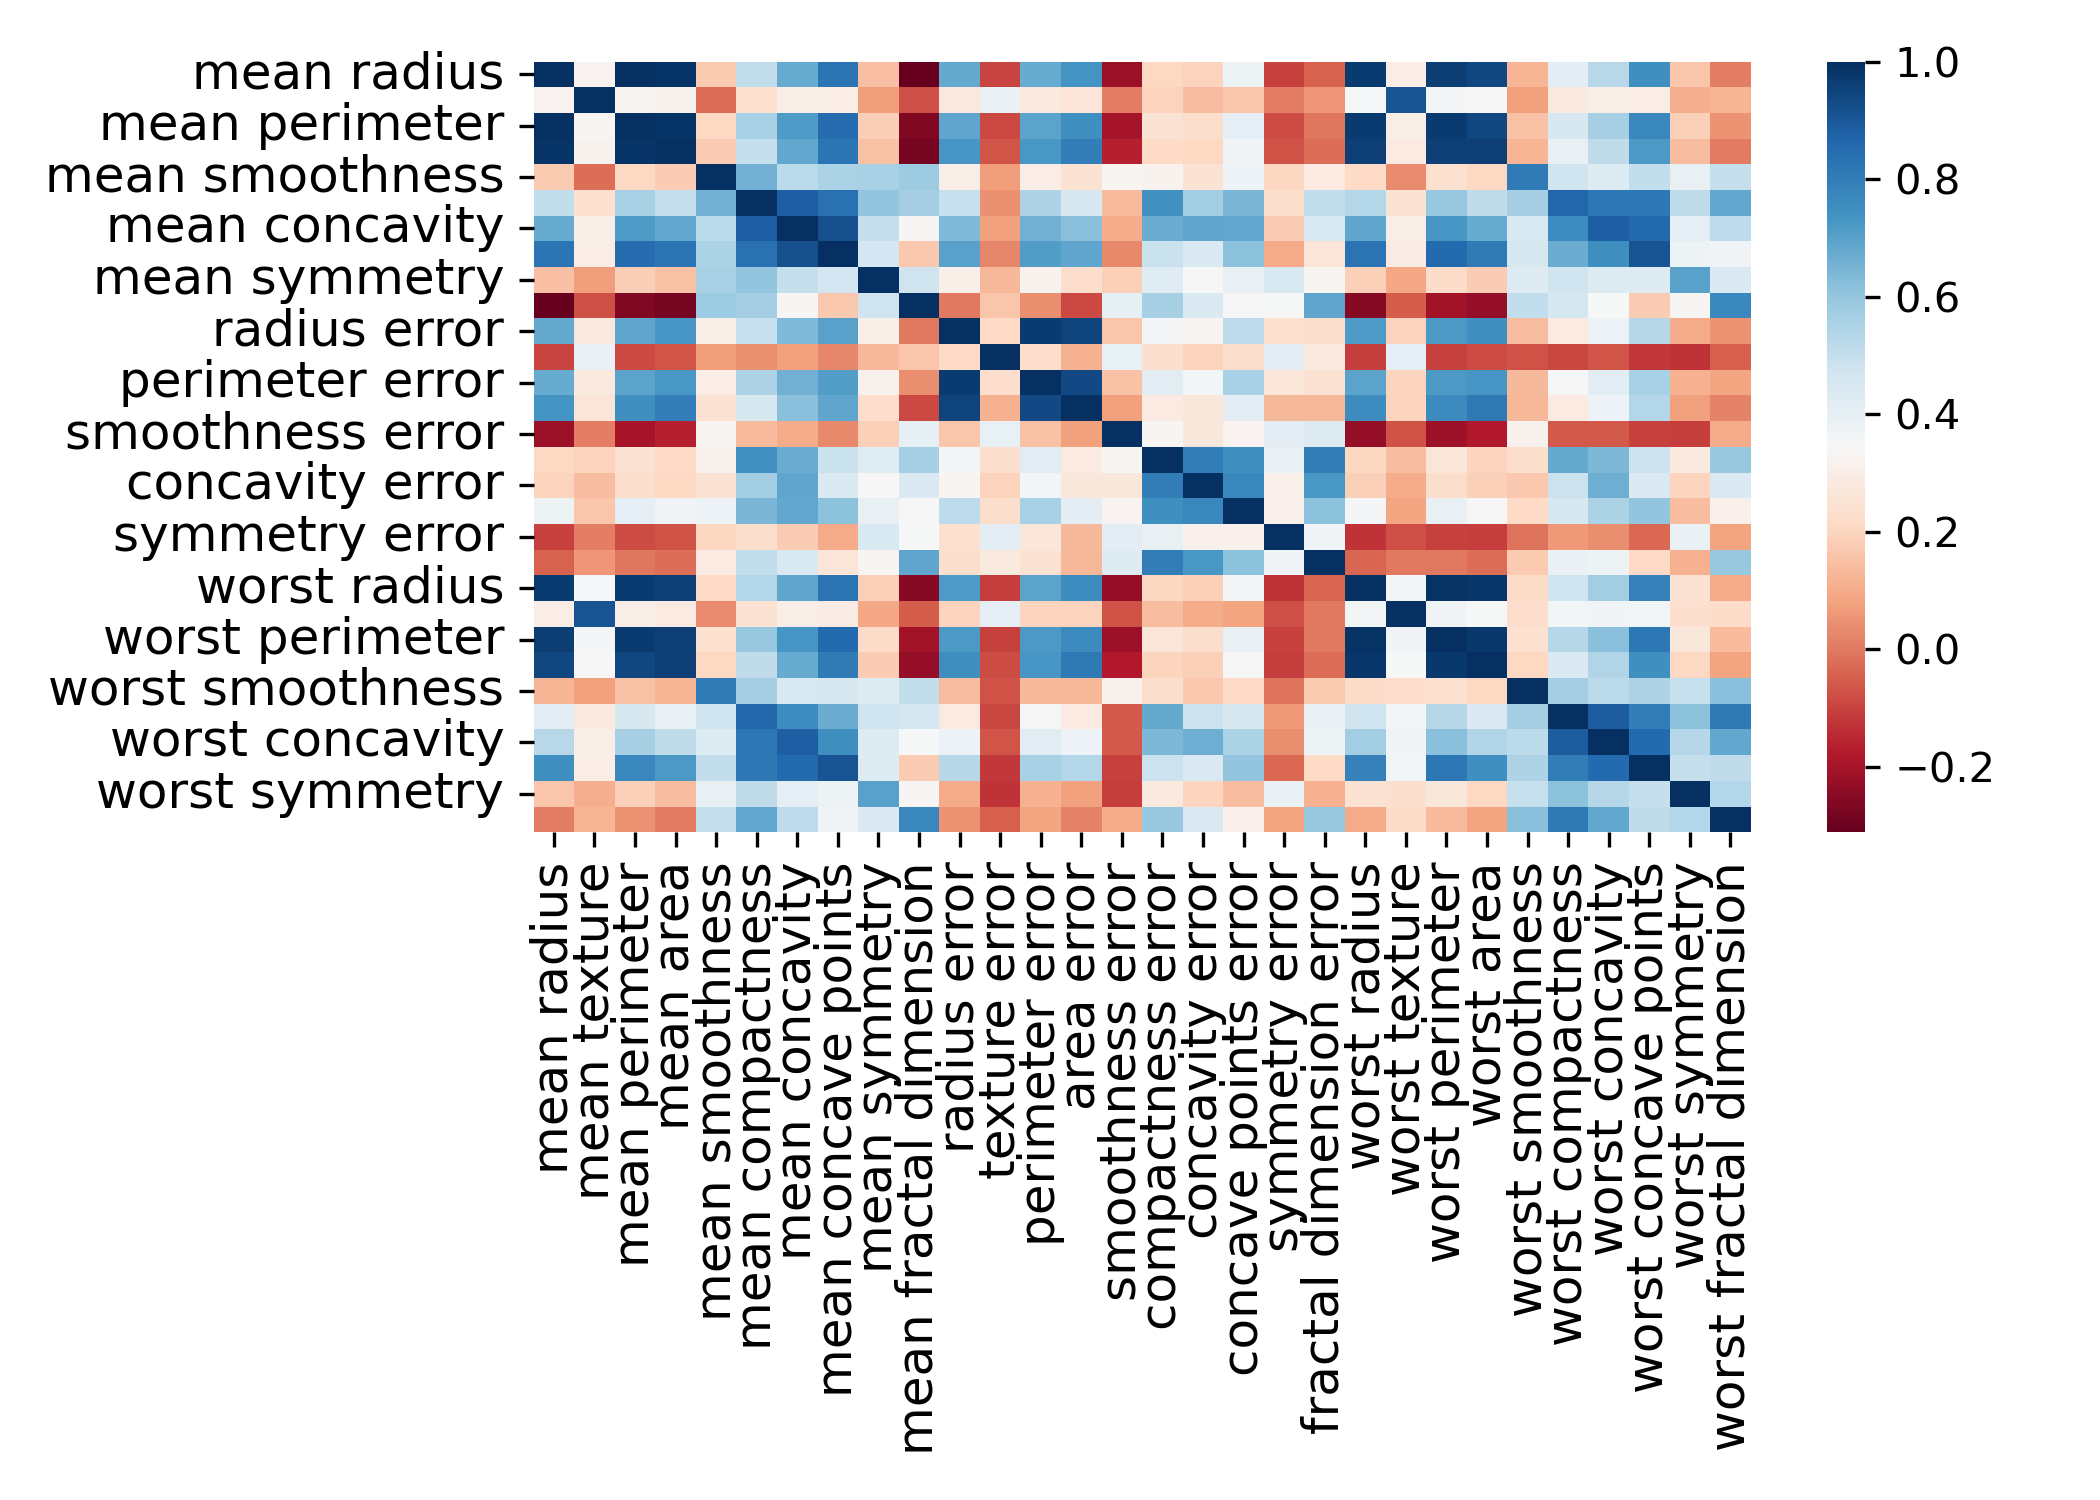
\includegraphics[width=0.98\textwidth]{images/scoreBasedAle/correlation_cancer.png}}
  \caption{Cancer data correlation map. Dark colors represent strong correlations.}
    \label{fig:correlation}
\end{figure}


\subsubsection{An inconsistency of TreeSHAP}

In the educational dataset examined, Figure \ref{fig:edu_data} illustrates that the \gls{MDI} exhibits greater density in its outputs compared to other metrics. Specifically, \gls{csPFI} and \gls{PFI} are the most sparse and exhibit high symmetry. Both metrics underscored features 29 (cumulative grade point average in the last semester) and 8 (salary) as paramount. Moreover, feature 29 emerged as a significant variable across multiple metrics. However, a discrepancy was observed between \gls{AUA} and TreeSHAP regarding the direction of this feature contribution. \gls{AUA} indicated a negative influence for feature 29, counter to domain knowledge, while TreeSHAP suggested a positive influence. To further scrutinize this divergence, we employed the original version of \gls{SHAP} (in red in Figure \ref{fig:edu_data}), which corroborated \gls{AUA}'s findings.

Furthermore, an additional logistic regression model further substantiated this negative effect with a statistically significant coefficient of -0.99. PD plots for both logistic regression and random forest models also corroborated this negative direction, raising evidence of the negative effect of feature 29 to this dataset. 

Upon closer analysis of the cross-validation process, it was observed that TreeShap assigns both positive and negative effects across iterations, a phenomenon not seen with other techniques. These changes in sign, depending on the fold, introduce noise into the final signal of relevance and diminish the overall relevance of the feature due to positive and negative cancellations.

The inconsistency observed in TreeSHAP might be related to its strategy of holding conditional expectations to avoid data extrapolation, as previously documented \cite{SilvaFilho2023AAchievement}. In a controlled experiment, the authors evaluated multiple algorithms using different metrics of feature contribution on a dataset where two features were identically correlated with the target variable and shared the same joint distribution. Despite these conditions, the two features received significantly different average feature contributions, but only in the TreeSHAP metric. This divergence arises from the different conditional expectations used to compute the effects of both features, even though they have exactly the same distribution. The conditional distribution used to compute feature effects depends on the specific terminal branches where the features are located within the decision trees. In this experiment, the small sample size and the repeated stochastic nature of random forest modeling likely contribute to this inconsistency across the 5-fold cross-validation process.

\subsubsection{The robustness of the ALE-based score}

In Figure \ref{fig:edu_data}, a dendrogram identifies a set of features highly correlated with Salary (feature 8), a variable widely acknowledged as a determinant of educational performance \cite{coleman1968equality, coleman2019equality}. This correlated group comprises features such as \textit{Transportation to the University} (9), \textit{Accommodation Type in Cyprus} (10), \textit{Mother's Education} (11), and\textit{ Parental Status} (14). Upon closer inspection of this cluster (highlighted in orange in Figure \ref{fig:edu_data}), it becomes evident that various techniques may accentuate correlated features, thereby introducing potential false positives. The \gls{MDI} metric distributes relevance broadly across the entire group, with \textit{Mother's Education} (11) emerging as the most significant. Conversely, other metrics, with the exception of TreeSHAP, align with domain knowledge and prioritize \textit{Salary} (8). Among these, \gls{PFI}, \gls{csPFI}, and \gls{AUA} appear to be more robust in isolating inter-feature dependencies within the group. TreeSHAP, however, probably erroneously attributes nearly equal importance to \textit{Accommodation Type in Cyprus} (10) as it does to \textit{Salary} (8), despite the former should not be directly related to educational performance.



\begin{figure}[ht!]
\centering
  \fcolorbox{gray}{white}{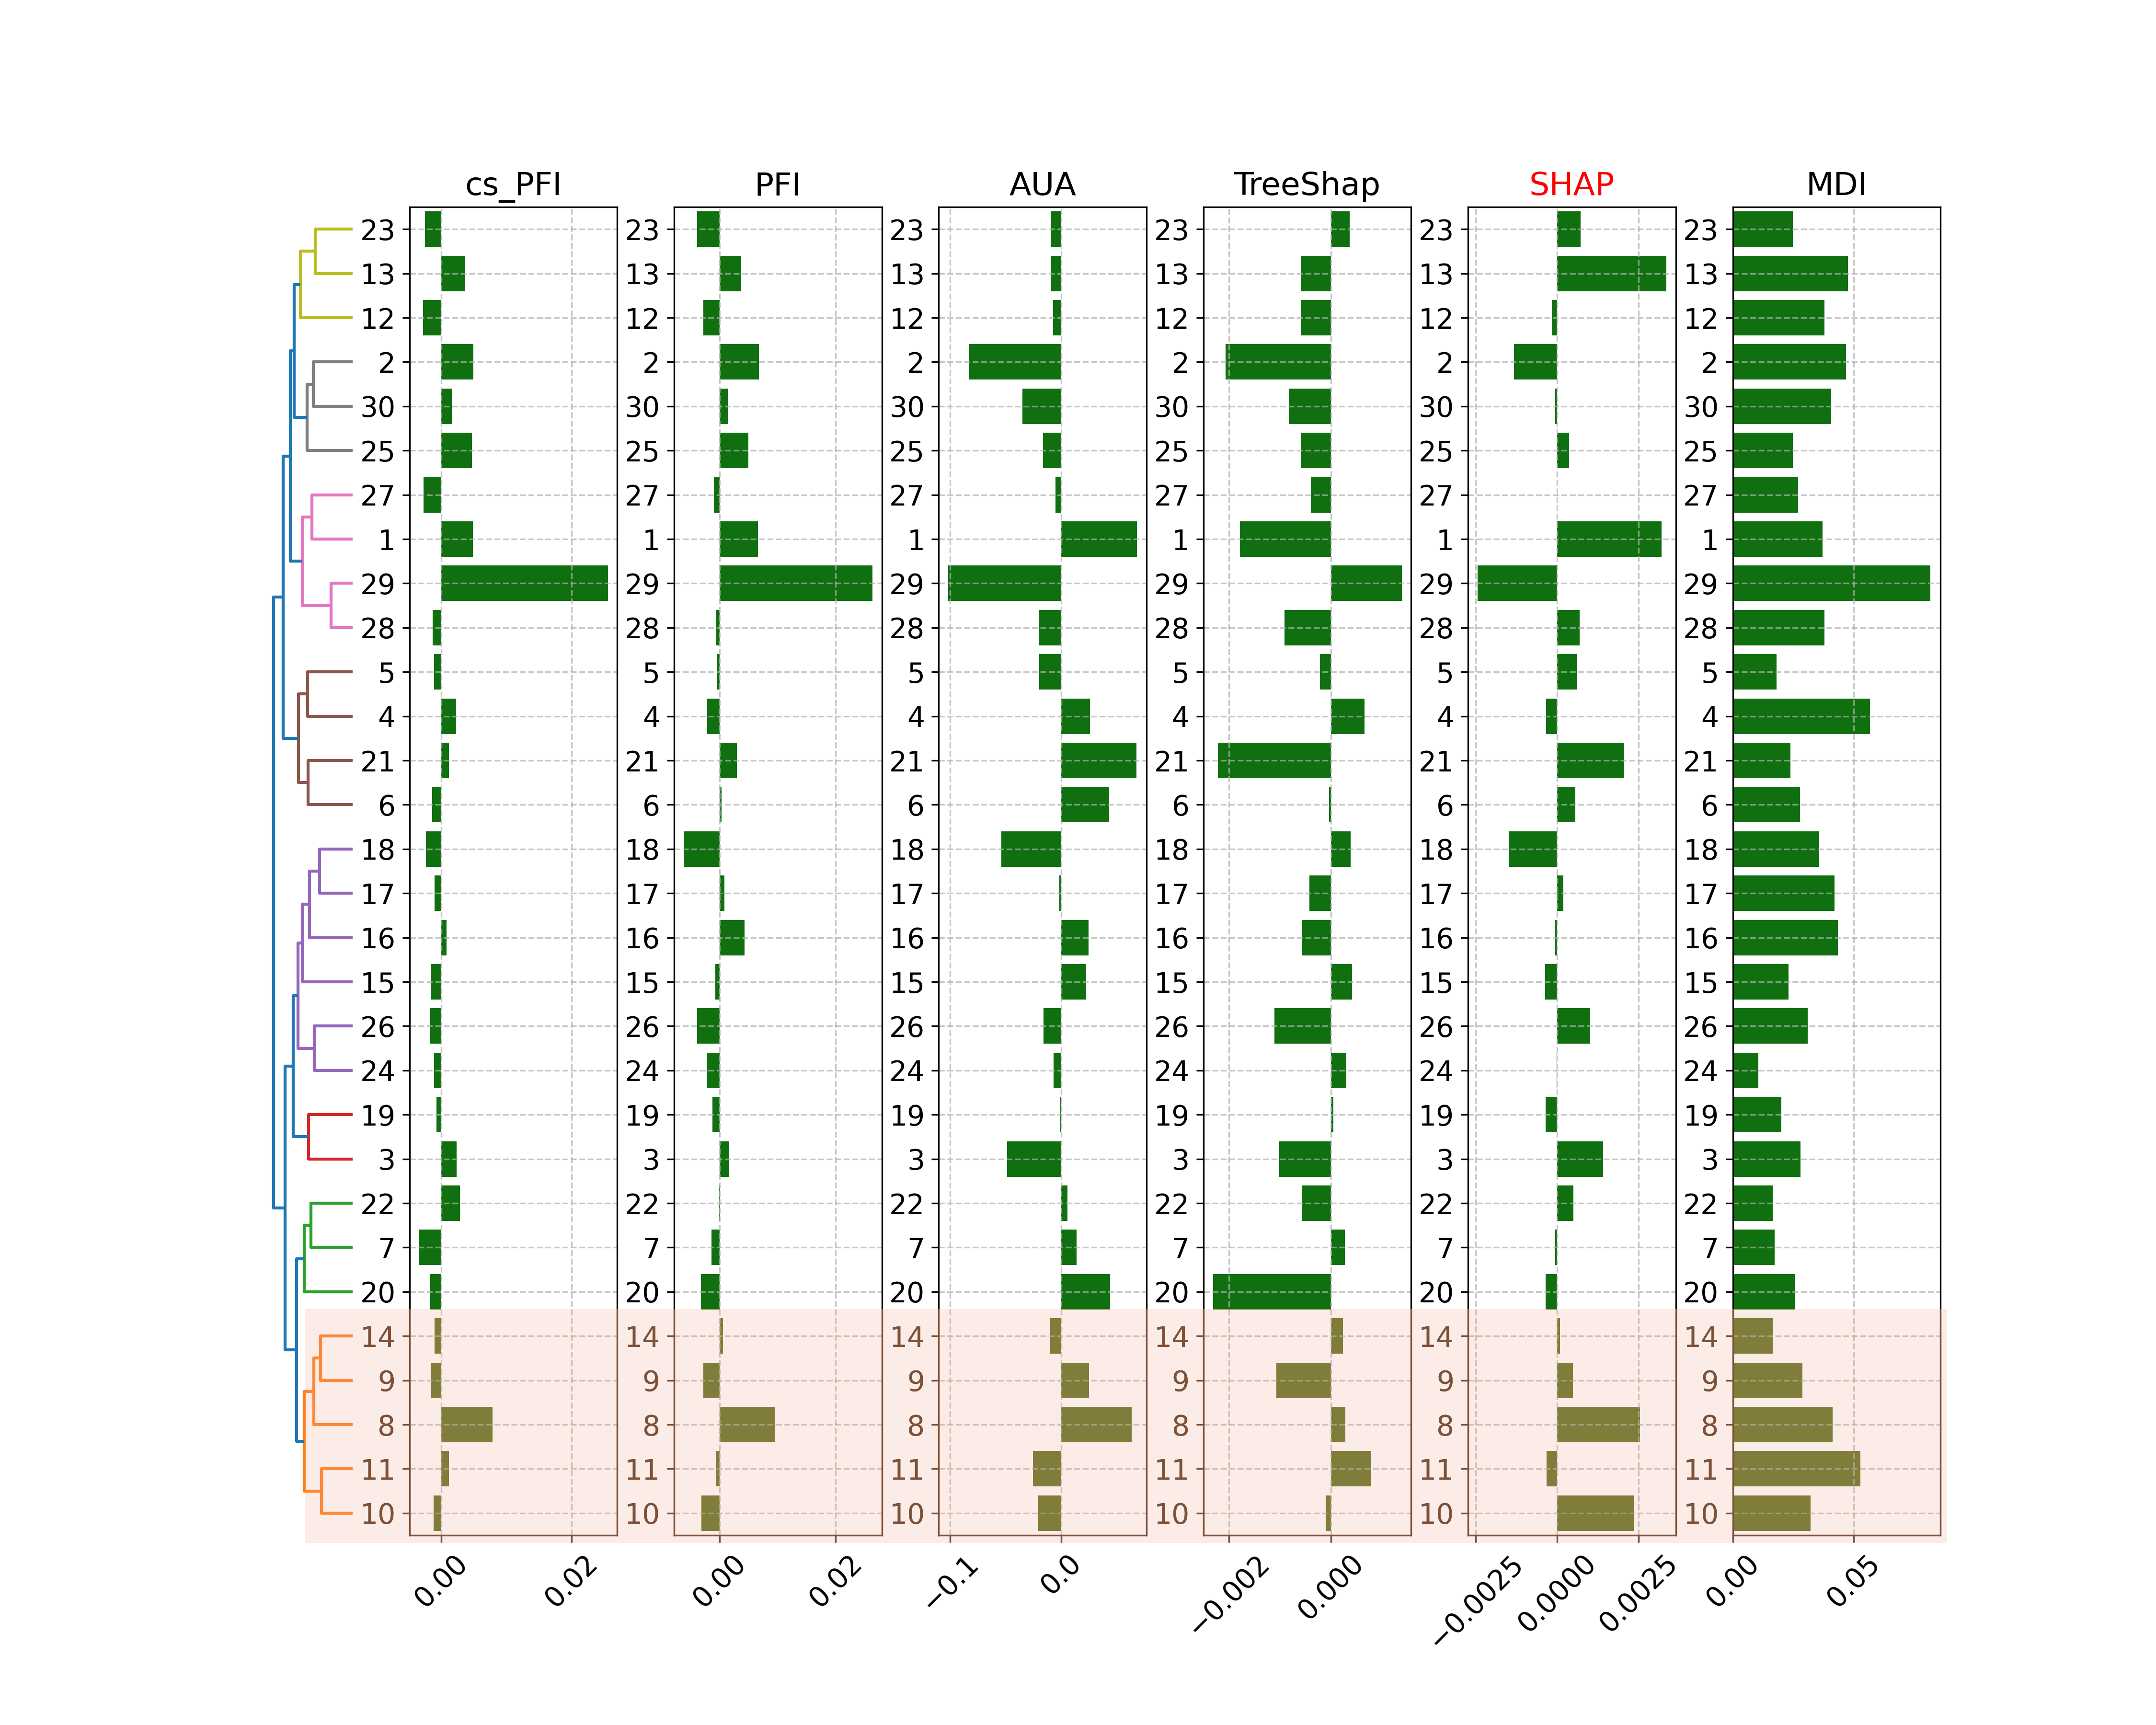
\includegraphics[width=0.98\textwidth]{images/scoreBasedAle/edu_data_edited.png}}
  \caption{Feature attribution to the educational data. The orange area highlights a cluster of features highly correlated to the Salary, as illustrated in the left dendrogram. The dendrogram was computed by using scipy package}
    \label{fig:edu_data}
\end{figure}

\footnote{\url{https://scipy.org/} using the complete linkage option.}

\subsection{Feature selection}

In assessing the efficacy of \gls{ALE}-based scores for feature selection, the \gls{AAR} proved effective, reducing model complexity without significantly impacting model performance, akin to the baseline \gls{MDI}. The initial experiment, utilizing educational data, underscored the benefits of \gls{AAR}, achieving a 28\% reduction in the number of features with only a slight impact on model performance. In contrast, despite the fact that \gls{MDI} had been built during random forest training and can have the full information about how the algorithm used features, it was less effective in reducing feature count, deeming only one variable as irrelevant (\(< 0.001\)). Notably, when comparing the performance of models using the top 10 variables identified by both scores, the results were consistent despite a disagreement in 4 variables within the top 10. The Table \ref{tbl:feature_selection_edu} presents these findings, showcasing outcomes for both logistic regression and random forest algorithms.

\begin{table}[ht]
\caption{Comparison between MDI from RF and the ALE-based score AAR for feature selection in an openly educational dataset to predict student drop-outs.}
\label{tbl:feature_selection_edu}
\centering
\rowcolors{1}{}{lightgray}
\begin{tabular}{l|c|c}
\toprule
Model & AUC\_ROC & Number of features \\
\midrule
Random Forest (All Features) & 0.91 & 36 \\
Random Forest (MDI Relevant Features) & 0.91 & 35 \\
Random Forest (AAR Relevant Features) & 0.90 & 25 \\
Random Forest (MDI Top 10 features) & 0.88 & 10 \\
Random Forest (AAR Top 10 Features) & 0.88 & 10 \\
\bottomrule
\end{tabular}
\end{table}



In the second series of experiments with OpenML datasets, the \gls{AAR} method effectively reduced the number of features. For dataset id=312, shown in Figure \ref{fig:opemML312}, reducing the number of features did not significantly boost the model's performance, as the \gls{AUC} remained stable for both \gls{AAR} and \gls{MDI} methods. However, \gls{AAR} was more successful in cutting down the number of features. In the initial threshold, \gls{AAR} reduced the number of features by 16\%, compared to \gls{MDI}'s reduction of 13\%. At the subsequent evaluated thresholds, \gls{AAR} achieved reductions of 44\% and 60\%, while \gls{MDI} achieved reductions of 26\% and 54\%, respectively.

With dataset id=1485, removing features led to better model performance. This aligns with earlier results, showing \gls{AAR}'s efficiency in simplifying the model without compromising its effectiveness, particularly up to a threshold of 0.002. At a threshold of 0.001, \gls{AAR} managed to reduce 20\% more features than \gls{MDI}. Notably, at a threshold of 0.03, \gls{MDI} performed better,  possibly due to its direct connection to the RF model used for fitting the data. To investigate this further, the RF model was replaced with a logistic regression model in the second step. The results are presented in Figure \ref{fig:opemML312_lr}. Using the logistic model, \gls{AAR} demonstrated even stronger results up to a 0.002 threshold, while \gls{MDI} continued to achieve greater feature reduction at the 0.003 threshold. However, as expected, the difference in performance at this threshold is now negligible.


\begin{figure}[ht!]
\centering
  \fcolorbox{gray}{white}{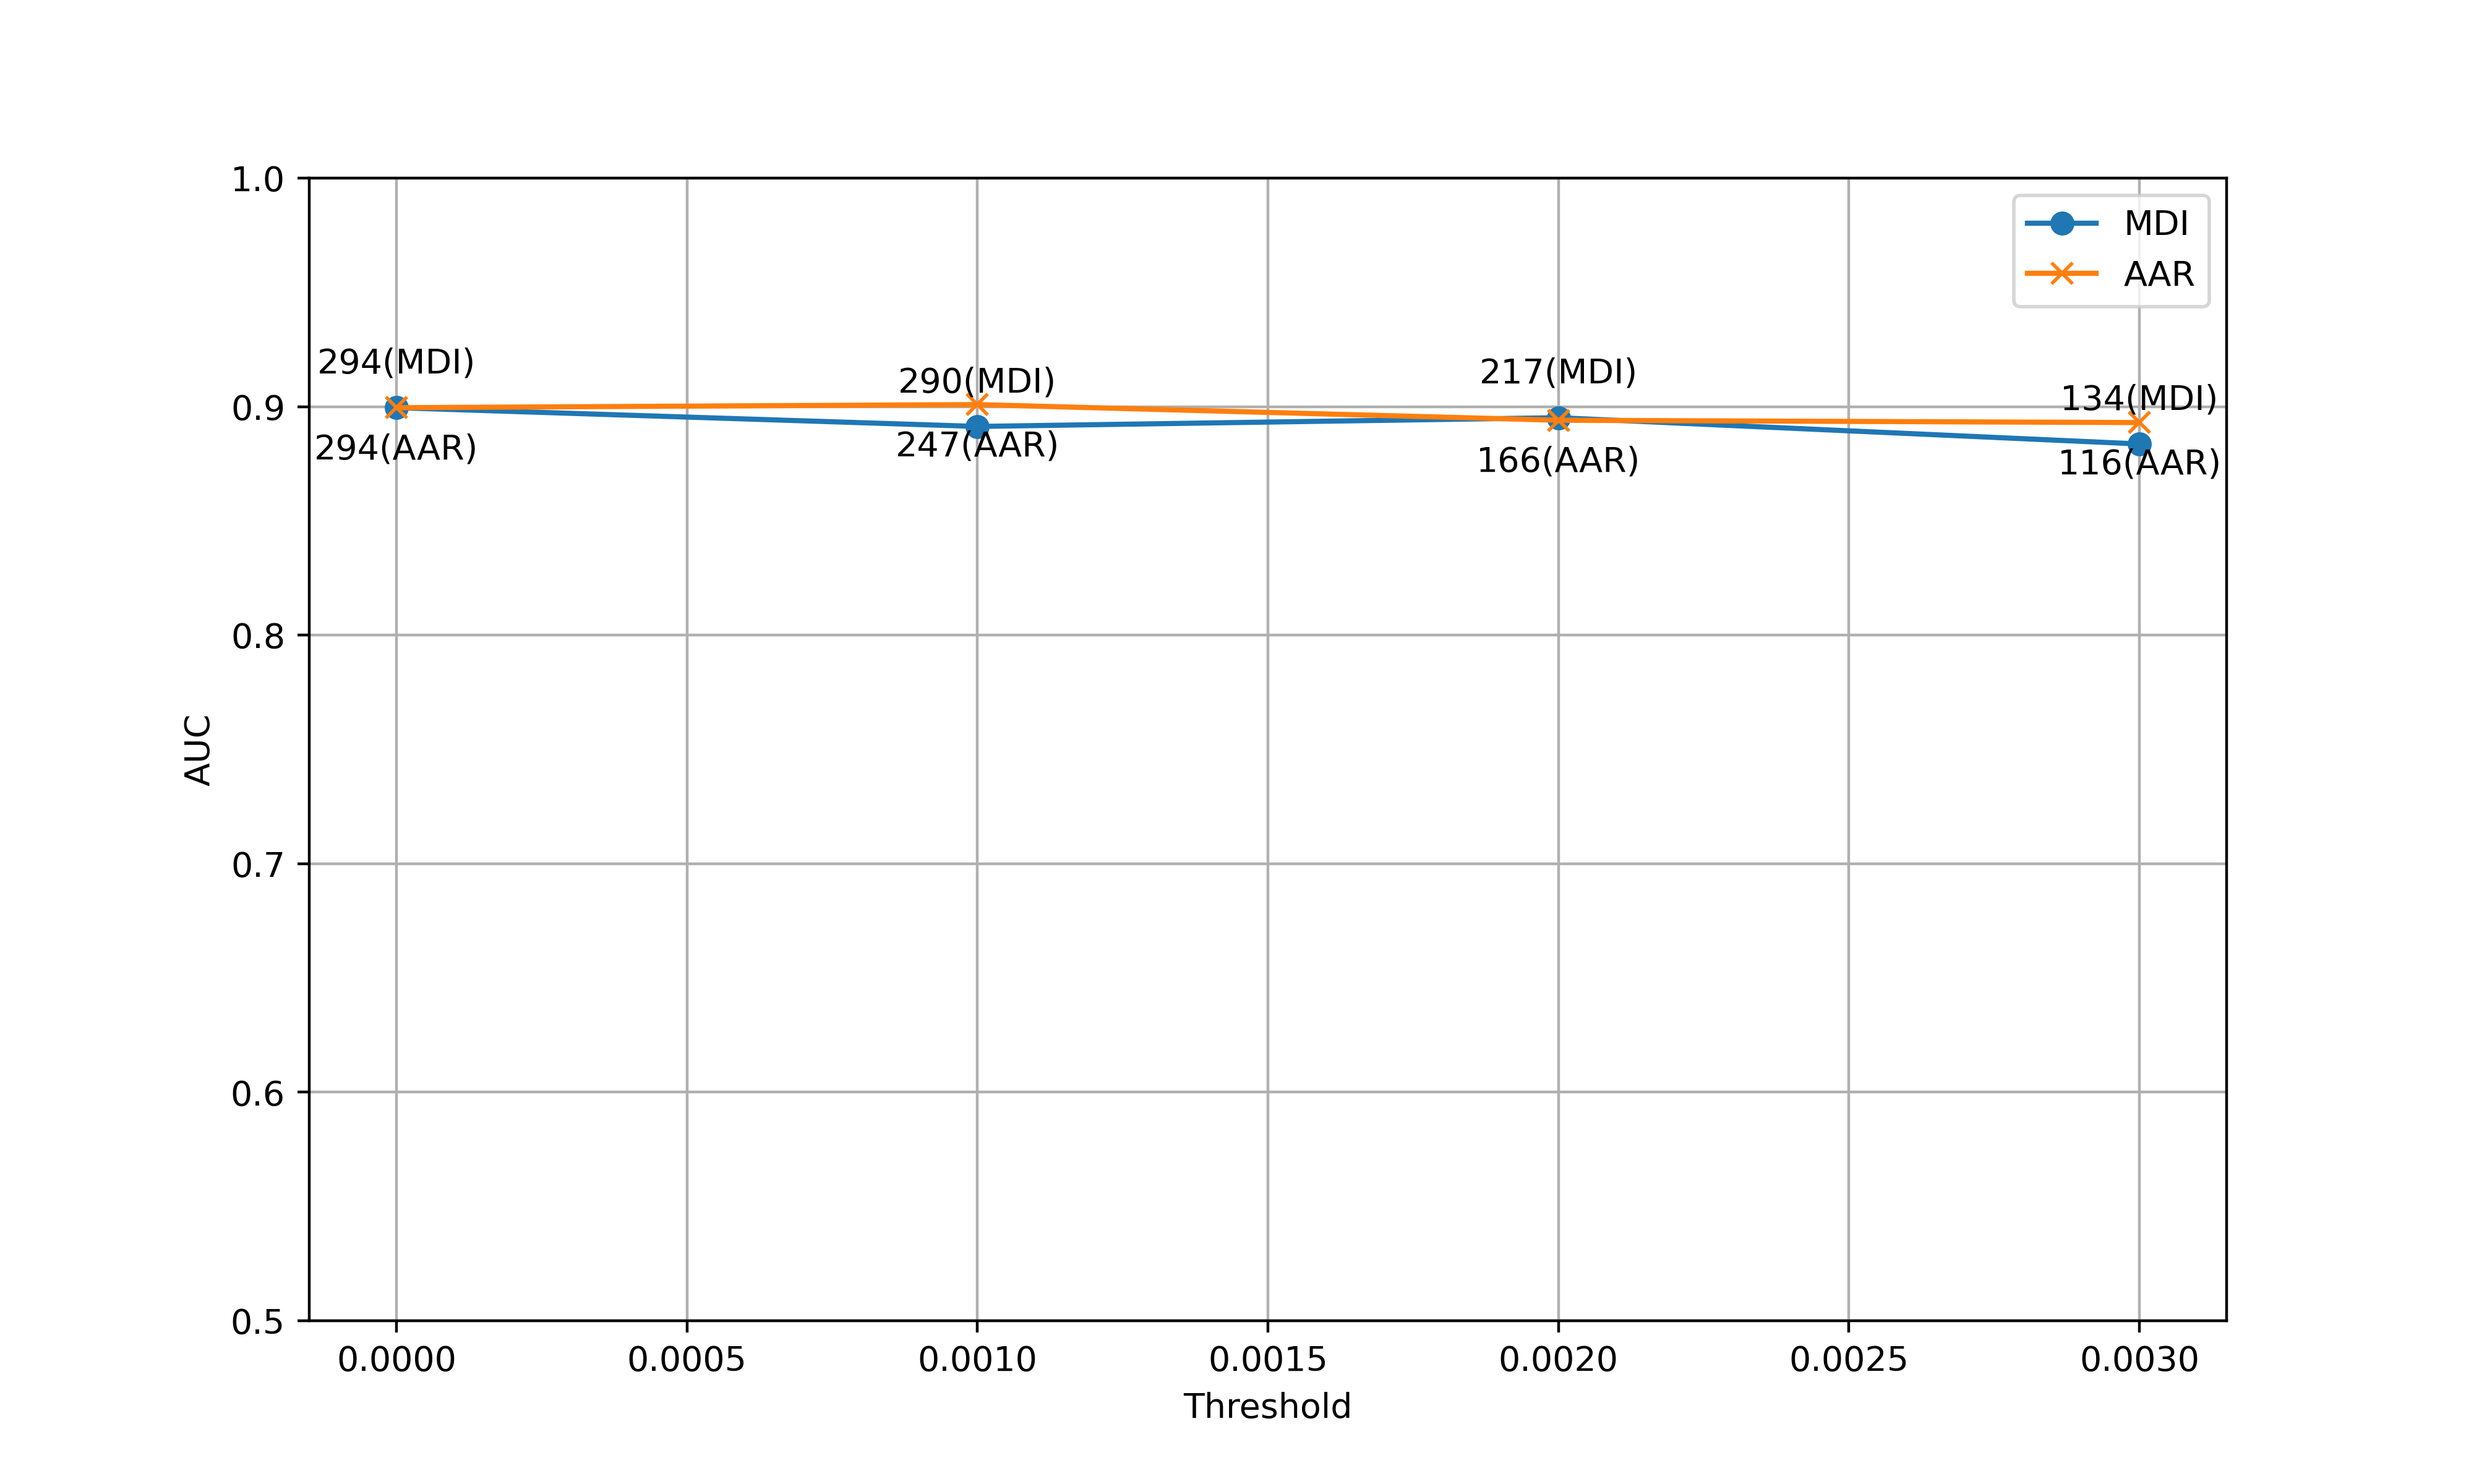
\includegraphics[width=0.98\textwidth]{images/newMetrics/feature_selection_openML312.png}}
  \caption{Comparative analysis of the ALE-based AAR score and MDI from RF in reducing model complexity by minimizing the number of features. The dataset is from OpenML (id=312) in a classification task. The number represents the number of remaining features on the dataset for each metric. }
    \label{fig:opemML312}
\end{figure}


\begin{figure}[ht!]
\centering
  \fcolorbox{gray}{white}{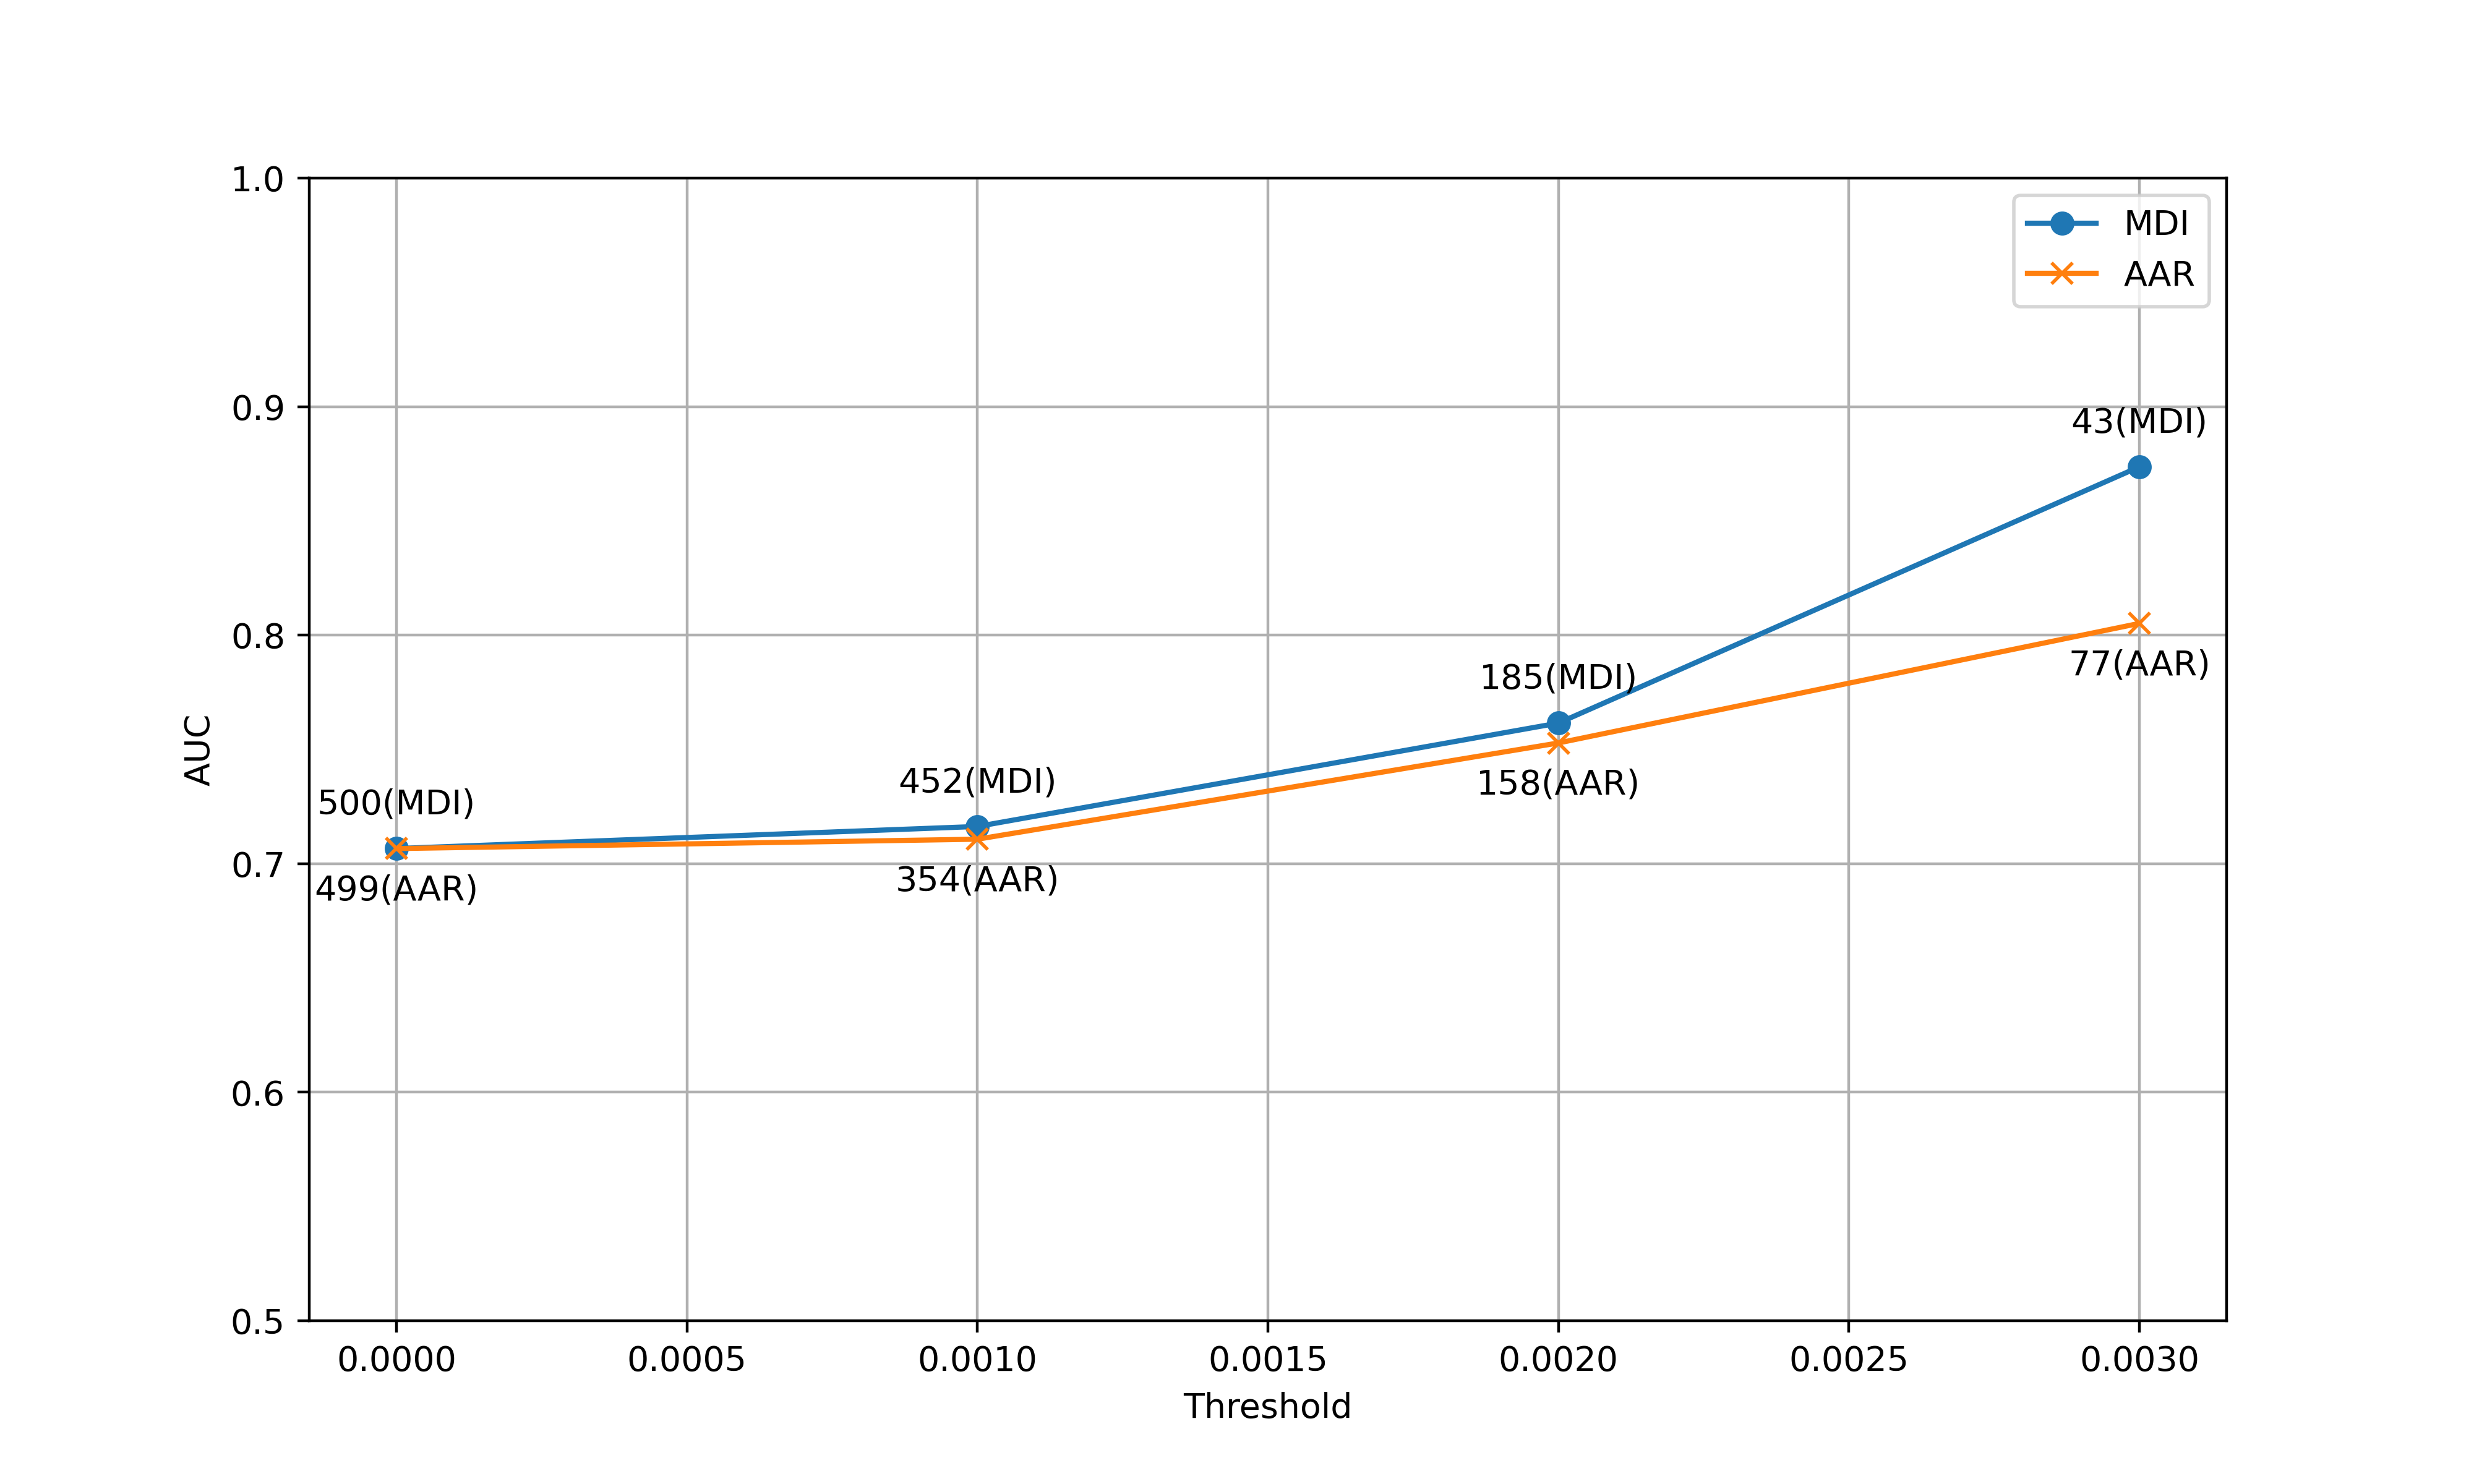
\includegraphics[width=0.98\textwidth]{images/newMetrics/feature_selection_openML1485.png}}
  \caption{Comparative analysis of the ALE-based AAR score and MDI from RF in reducing model complexity by minimizing the number of features. The dataset is from OpenML (id=1485) in a classification task. The number represents the number of remaining features on the dataset for each metric.}
    \label{fig:opemML312}
\end{figure}

\begin{figure}[ht!]
\centering
  \fcolorbox{gray}{white}{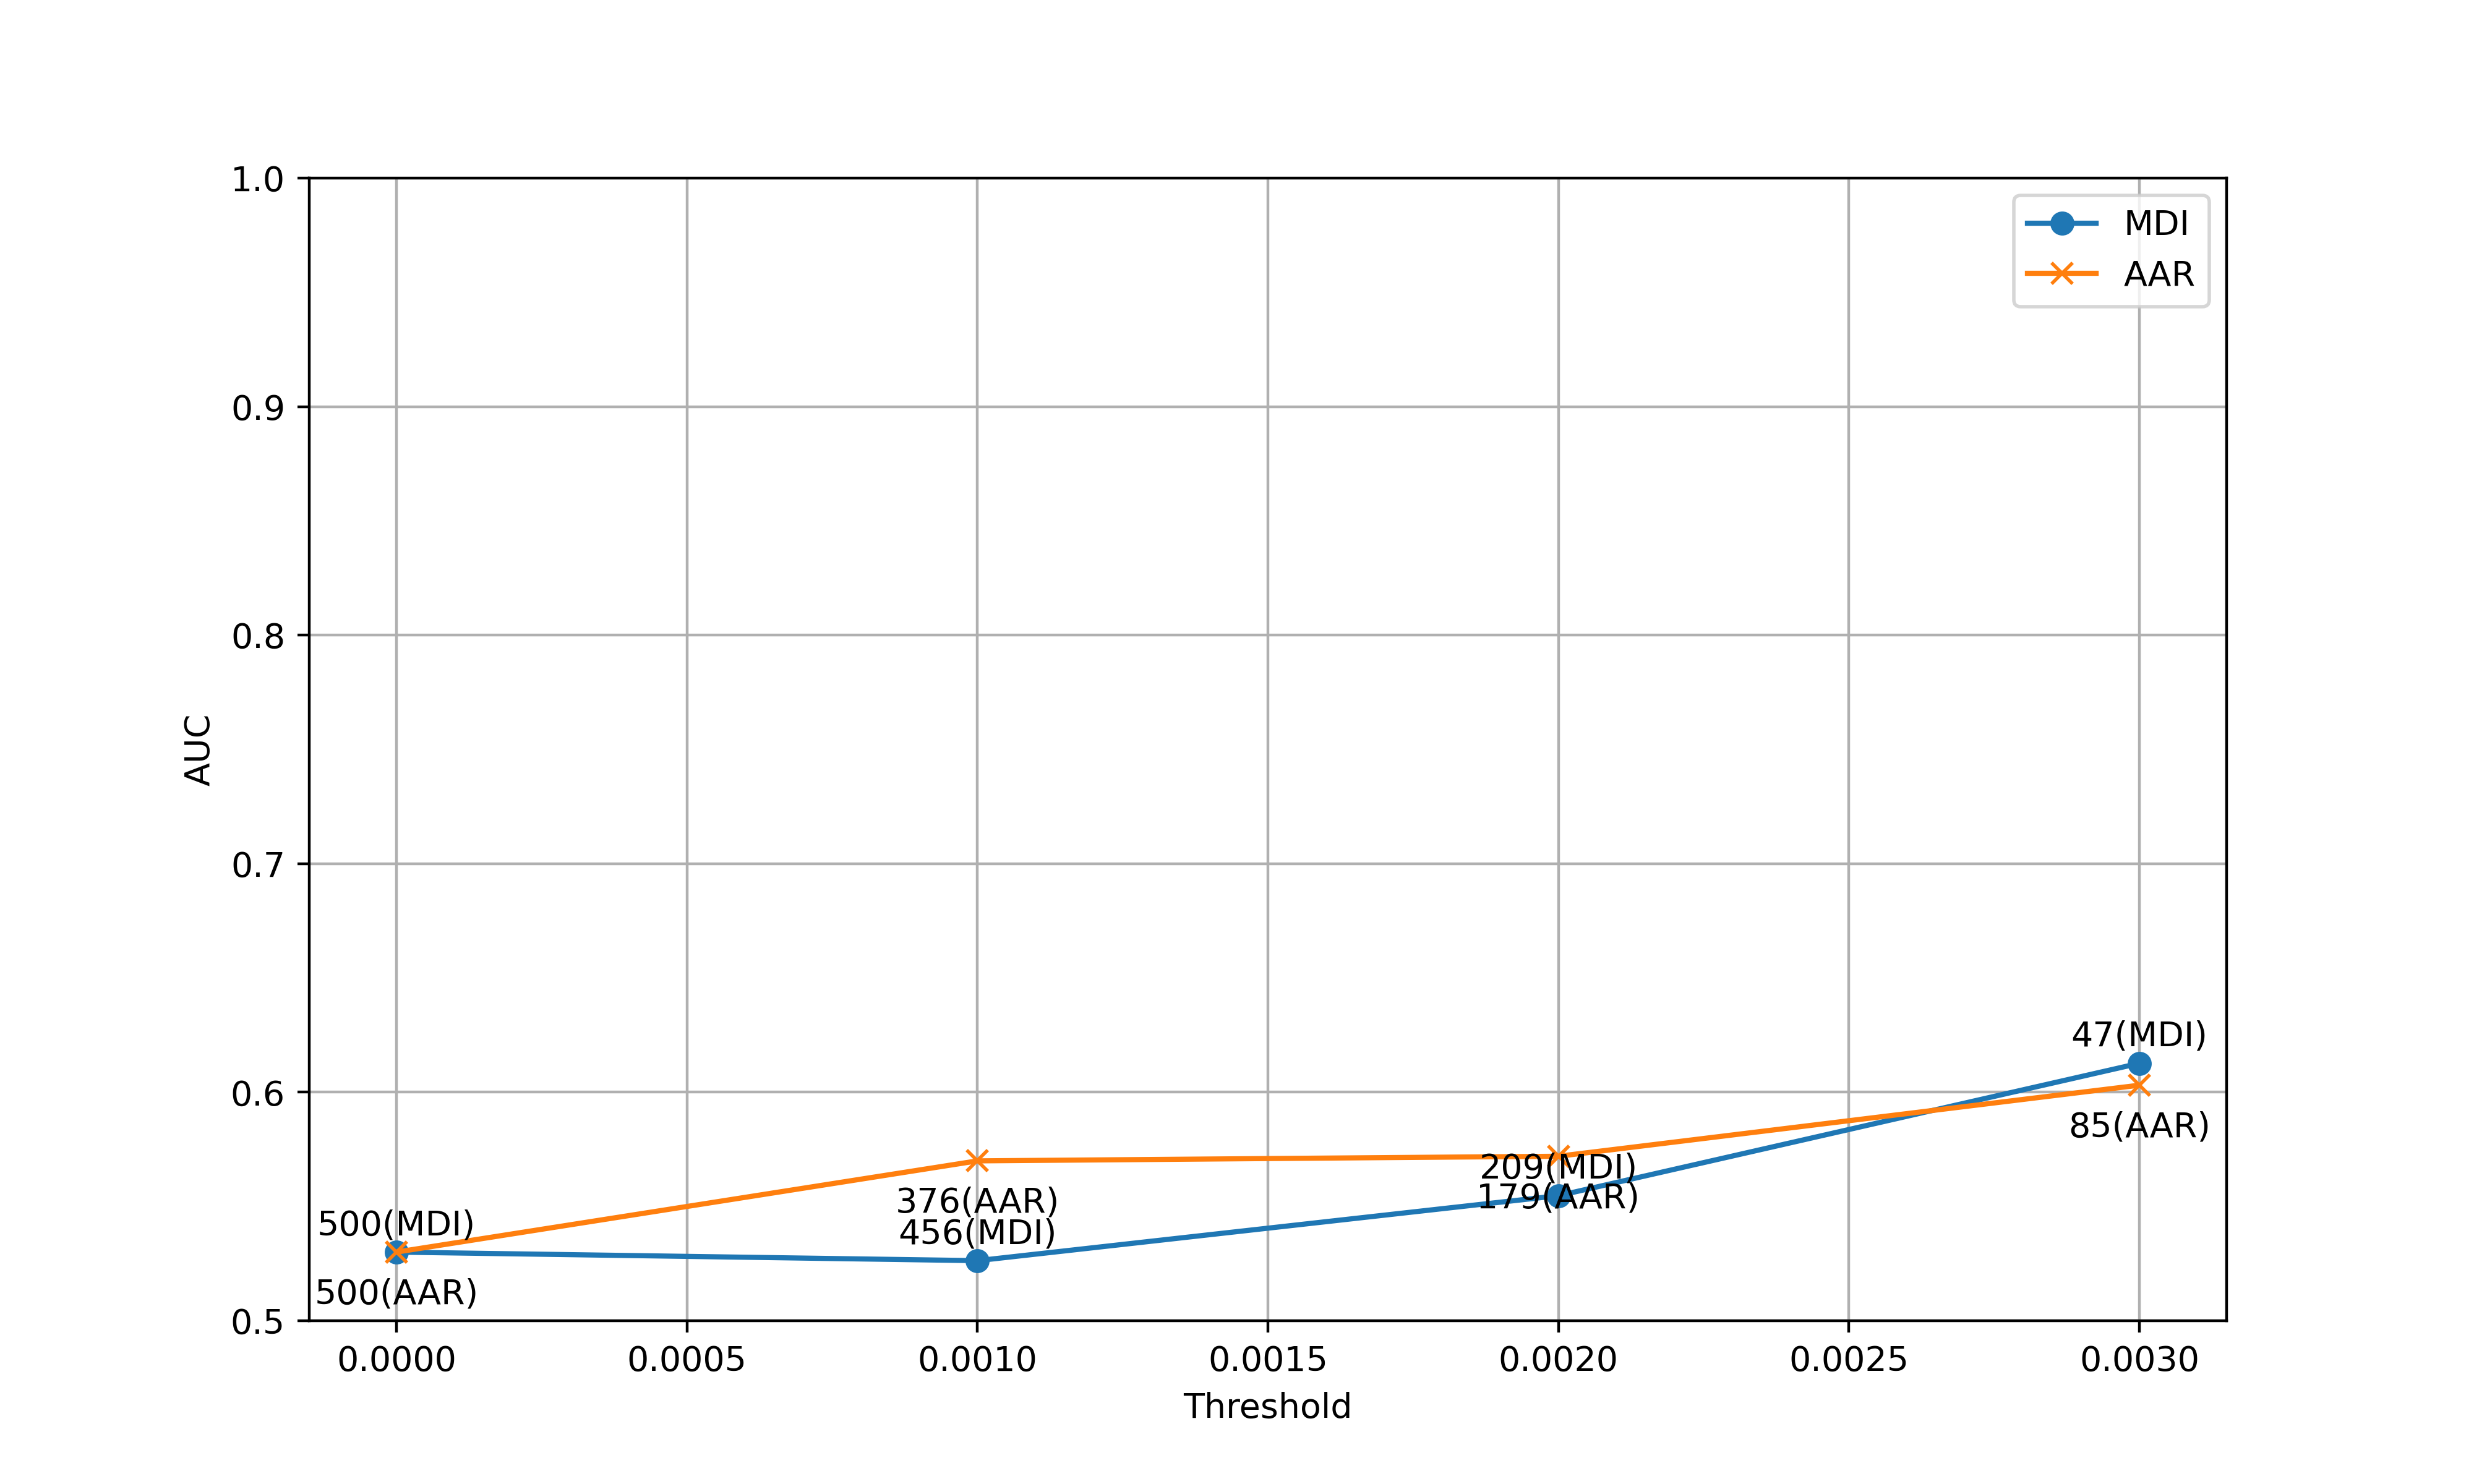
\includegraphics[width=0.98\textwidth]{images/newMetrics/feature_selection_openML1485)lr.png}}
  \caption{Comparative analysis of the ALE-based AAR score and MDI from RF in reducing a \textbf{logistic regression} model complexity by minimizing the number of Features. The dataset is from OpenML (id=1485) in a classification task. The numbers represent the number of remaining features on the dataset for each metric.}
    \label{fig:opemML312_lr}
\end{figure}




